%%%%%%%%%%%%%%%%%%%% author.tex %%%%%%%%%%%%%%%%%%%%%%%%%%%%%%%%%%%
%
% sample root file for your "contribution" to a contributed volume
%
% Use this file as a template for your own input.
%
%%%%%%%%%%%%%%%% Springer %%%%%%%%%%%%%%%%%%%%%%%%%%%%%%%%%%


% RECOMMENDED %%%%%%%%%%%%%%%%%%%%%%%%%%%%%%%%%%%%%%%%%%%%%%%%%%%
\documentclass[graybox]{svmult}

% choose options for [] as required from the list
% in the Reference Guide

\usepackage{mathptmx}       % selects Times Roman as basic font
\usepackage{helvet}         % selects Helvetica as sans-serif font
\usepackage{courier}        % selects Courier as typewriter font
\usepackage{type1cm}        % activate if the above 3 fonts are
                            % not available on your system
%
\usepackage{makeidx}         % allows index generation
\usepackage{graphicx}        % standard LaTeX graphics tool
                             % when including figure files
\usepackage{multicol}        % used for the two-column index
\usepackage[bottom]{footmisc}% places footnotes at page bottom
\usepackage{url}
%%%%%%%%%%%%%%%%%%%%%%%%%%%%%%%%%%%%%%%%%%%%%%%%%%%%%%%%%%%%%%%%%%%

\usepackage{amsfonts}		% math fonts.


% see the list of further useful packages
% in the Reference Guide

\makeindex             % used for the subject index
                       % please use the style svind.ist with
                       % your makeindex program

%%%%%%%%%%%%%%%%%%%%%%%%%%%%%%%%%%%%%%%%%%%%%%%%%%%%%%%%%%%%%%%%%%%%%%%%%%%%%%%%%%%%%%%%%

\newcommand{\Pow}{\mathcal{P}}
\newcommand{\N}{\operatorname{N}}
\newcommand{\bool}{\operatorname*{\mathcal{B}}}
\newcommand{\Pos}{\operatorname{Pos}}
\newcommand{\Nec}{\operatorname{Nec}}
\newcommand{\T}{\mathcal{T}}

\begin{document}

\title*{An overview on temporal databases.\\
 New approaches and proposals.}
% Use \titlerunning{Short Title} for an abbreviated version of
% your contribution title if the original one is too long
\author{Jos\'e Pons \and Christophe Billiet \and Olga Pons}
% Use \authorrunning{Short Title} for an abbreviated version of
% your contribution title if the original one is too long
\institute{Jos\'e Pons \at Department of Computer Science and Artificial Intelligence, Univeristy of Granada, C/ Periodista Daniel Saucedo Aranda s/n \email{jpons@decsai.ugr.es}
\and Christophe Billiet \at Department of Telecommunications and Information Processing, Ghent University, Belgium, St.-Pietersnieuwstraat 41, B-9000 Gent,Belgium. \email{Christophe.Billiet@telin.ugent.be}
\and Olga Pons \at Department of Computer Science and Artificial Intelligence, Univeristy of Granada, C/ Periodista Daniel Saucedo Aranda s/n \email{opc@decsai.ugr.es}
}
%
% Use the package "url.sty" to avoid
% problems with special characters
% used in your e-mail or web address
%
\maketitle

\abstract*{There exist some objects in the nature that have a time-variant (e.g. an employee's working life) or time-related (e.g. the transactions in a bank account) nature. Modelling these objects in a (relational) database is possible, but the time-related attributes have an impact on the consistency of the entire database. Therefore, some temporal database models have been proposed to deal with this. These models deal both with the problem of representation and querying. Time itself is a source of imprecision / vagueness / uncertainty since the measures of time are inherently imprecise. Humans beings manage the time with imprecision and vagueness. Nevertheless, the amount of uncertainty in the temporal indications are defined by socially well-known boundaries. Several proposals for dealing with imprecision in time have been done: some proposals consider the basis of the system the imprecision related to the conversion of diferent time points and intervals. While some other proposals consider the specification of the time as the source of imprecision: the time points are ill-known.}

\abstract{There exist some objects in the nature that have a time-variant (e.g. an employee's working life) or time-related (e.g. the transactions in a bank account) nature. Modelling these objects in a (relational) database is possible, but the time-related attributes have an impact on the consistency of the entire database. Therefore, some temporal database models have been proposed to deal with this. These models deal both with the problem of representation and querying. Time itself is a source of imprecision / vagueness / uncertainty since the measures of time are inherently imprecise. Humans beings manage the time with imprecision and vagueness. Nevertheless, the amount of uncertainty in the temporal indications are defined by socially well-known boundaries. Several proposals for dealing with imprecision in time have been done: some proposals consider the basis of the system the imprecision related to the conversion of diferent time points and intervals. While some other proposals consider the specification of the time as the source of imprecision: the time points are ill-known.}

\section{Introduction}
\label{sec:introduction}
%%%%%%%%%%%%%%%%%%%%%%%%%%%%%%%%%%%%%%%%%%%%%%%%%%%%%%%%%%%%%%%%%%%%%%
%
% Introduction
%
%%%%%%%%%%%%%%%%%%%%%%%%%%%%%%%%%%%%%%%%%%%%%%%%%%%%%%%%%%%%%%%%%%%%%%

The concept of time is very complex to handle and interpret~\cite{Klein1994,Shackle1961}, though it is very natural and omnipresent in real world data. As information systems attempt the modelling of natural objects, concepts or processes, they often require modelling temporal aspects or concepts. Thus, several proposals have arisen to obtain theoretical models that allow the modelling or representation of time~\cite{Bolour1982,VanderCruyssen1997}.

A very specific type of information systems are database systems. A database contains data representing real objects or concepts. In real world, some aspects or properties of objects are time-variant or time-related. e.g., the moment of a bank transaction and the status of an employee in a company, are time-related and time-variant notions, respectively.
A temporal database schema is a database schema that models objects with time-related or time-variant properties. However, the modelling of temporal aspects has a direct impact on the consistency of the temporal database, because the temporal nature of these aspects imposes extra integrity constraints and suitable ways of interactive with the human user. 

For example, let us consider a hospital database containing data about the state of the patients in a given hospital. Two dates are stored: the date when the patient arrives to and leaves from the hospital. It is clear that a patient cannot leave the hospital if he or she has not arrived. Without further cautions, a hospital employee could insert a patient who is already in the hospital. A temporal database model will typically constrain record insertion and prevent similar modelling inconsistencies.

A lot of research concerns temporal database models and their approaches to the modelling of time. The first efforts were towards the representation of historical information related to objects represented by records in a database~\cite{Clifford1985}. Some proposals tried to extend the Entity Relationship Model~\cite{Klopprogge1983}, without impact on any database standards like SQL~\cite{Sarda1990}.

Notably, in 1994, ``A Consensus Glossary of Temporal Database Concepts'' was published~\cite{Dyreson1994}. For this publication, 44 temporal database researchers, among them, some of the main researchers in this field, cooperated to reach a consensus on the nature and definitions of some of the main temporal database concepts and terminology. This glossary was updated in 1998~\cite{Dyreson1998}.


% %From time in general to time in information systems
% In real world, some aspects or properties of objects, concepts or processes are time-variant or time-related. For example, the moment of a bank transaction is traditionally a point in time and thus a time-related notion, the function of an employee in a company can change through recorded history and is thus time-variant.  As information systems often attempt the modelling of natural objects, concepts or processes, they often require modelling temporal aspects or concepts. Thus, several proposals have been concerned with obtaining theoretical models that allow the modelling or representation of time~\cite{Bolour1982},~\cite{VanderCruyssen1997}.

% %From time in information systems to time in temporal databases
% Time is a complex concept, which makes modelling time in database systems complex too. A \emph{temporal database} is a database that deals with certain time-related aspects in its schema: a \emph{temporal database schema}~\cite{Dyreson1994} is a database schema that models entities (and interactions or relationships between entities) with time-related or time-variant properties. However, the modelling of temporal properties or aspects has a direct impact on the consistency of the resulting temporal database, because the temporal nature of these aspects or properties imposes extra integrity constraints. An example. Consider a relation in a relational library database, representing the physical absence (or presence) of books in the library. Every physical book is represented by a unique identifier. Every record in the relation contains such an identifier, a date on which the corresponding book was loaned and a date on which it was subsequently returned (if it was returned). As such, every record represents a period of time during which the physical book corresponding with the identifier is loand to a library customer. Without further precautions, a library employee could add several records with the same book identifier, different `loaned'-dates and no `returned'-dates. This group of records would represent the same physical book being loaned several times on different dates and never returned, which is of course impossible. A temporal database model will typically constrain record insertion and prevent similar modelling inconsistencies.

An interesting issue in temporal modelling concerns relationships between temporal notions. In this sense, Allen~\cite{Allen1983} studied temporal relationships between time intervals (and as a special case time points). Among others, the querying of temporal databases has greatly profited from these temporal relationships, because they allowed more powerful user-specified temporal query demands, by allowing to express more complex relationships between the temporal notions in the temporal expressions in the query. For example, a query like `who were the department heads when Thomas worked for the institution' can be evaluated using operators similar to Allen's ones.

Humans handle temporal information using certain temporal notions like time intervals or time points~\cite{Dyreson1994}, and they often have to deal with imperfections like imprecision, vagueness, uncertainty or inconsistencies possibly contained in the descriptions of these temporal notions. These possible imperfections in descriptions of temporal notions determine an important issue in temporal modelling. Consider as an example the description of the temporal notion in a sentence like `The Belfry of Bruges was finished between 01/01/1201 A.D. and 31/12/1300 A.D.'. These sentence contains imperfection because of the uncertainty in the used time-related expression. It is known that the building was finished on a single day, but this day is not precisely known.

To allow information systems to cope with these and similar data imperfections, many approaches adopt fuzzy sets~\cite{Zadeh1965} for the representation and management of temporal information~\cite{Mitra1994,Nagypal2003,Billiet2011,Dubois2003}. The temporal relationships studied by Allen were fuzzified by several authors~\cite{Ohlbach2004,Nagypal2003,Schockaert2008}.   Garrido et al. ~\cite{Garrido2009} presented a compact representation for the time and defined different relationships among time intervals by using a combination of regular fuzzy comparisons. Also ~\cite{Garrido2009,Pons2011} studied uncertainty in temporal expressions concerning time intervals. Other approaches, like~\cite{Qiang2009}, use rough sets~\cite{Pawlak1995} to represent time intervals.

%Now introducing imperfections in representations of time...
% Humans handle temporal information using certain temporal notions like specific time intervals or instants~\cite{Dyreson1994} and they often have to deal with imperfections like imprecisions, vaguenesses, uncertainties or inconsistencies possibly contained in (the descriptions of) these temporal notions. Among many others, these possible imperfections in (descriptions of) temporal notions determine an important issue in temporal modelling. As an example, consider the temporal notion described in a sentence like `The Belfry of Bruges was finished on a day somewhere between 01/01/1201 A.D. and 31/12/1300 A.D.'. The description of the temporal notion reads `a day somewhere between 01/01/1201 A.D. and 31/12/1300 A.D.'. This temporal notion thus contains imperfection in the form of the uncertainty about the exact day the last stone of the building was laid: it is known that the building was finished on a single day, but it is not known which day this was. To allow information systems to cope with these and similar temporal data imperfections, many approaches adopt fuzzy sets~\cite{Zadeh1965} and/or fuzzy logic to model temporal information~\cite{Mitra1994},~\cite{Nagypal2003},~\cite{Billiet2011},~\cite{Dubois2003}. 

In addition to temporal modelling, some attention has been paid to temporal reasoning~\cite{Allen1983}. Although temporal reasoning is not discussed in this paper, it should be noted that, among others, Dubois and Prade et al.~\cite{Dubois2003,DuBois1989} have dealt with fuzziness and uncertainty in temporal reasoning.

The present work defines and implement a model for properly represent and manage uncertainty in valid-time specification in a relational database. Our work is focused on both the proposal of an appropriate formal framework to suitably manage time in databases and the implementation of an DML that allows to the user the transparent use of this proposal. None of the previous research offer a database model to accomplish this task.

This way together with the theoretical model, we also present and explain the main operations of the manipulation language for a temporal database which stores the valid-time periods of the objects affected by imprecision. The rest of the work is organized as follows. Section \ref{sec:prelim} presents some background concepts about both possibility theory and temporal databases. In section \ref{sec:time-rep} the representation of the valid-time intervals in the database is explained. Section \ref{sec:temporal-model} explains the main concepts of the temporal Data Manipulation Language (DML) and its implementation. Finally, Section \ref{sec:conclusions} presents the conclusions and some guidelines for future research work.


% 
% 
% %From information systems in general to database systems in particular:
% Generally, \emph{information systems} model the structure and behavior of real objects, concepts or processes. A specific type of information systems are \emph{database systems}, which are computer systems designed to manage \emph{databases}. A database is basically a collection of (persistent) data. These (typically atomic) data represent real objects or concepts. In the context of database design, such objects or concepts are typically called \emph{entities} and a collection of similar entities is typically modelled by an \emph{entitytype}, which is basically a combination of a name and a list of \emph{attributes}, which describe properties of the entities. Typically, in an early stage of the database development process, the structures of and interactions or relationships between used entities are modelled in a \emph{design schema}, following some design model. A database thus contains (typically atomic) data. Each (atomic) part of these data is a result value of a measurement of a property of an entity or a description of a property of an entity and will correspond to the attribute of the entity's entitytype, which describes the property.
% 
% %From database models in general to the relational model in particular:
% The structure and behavior of a database, along with some integrity and security restrictions, is dictated by a \emph{database model}. A database model is basically a collection of instructions and regulations, used to (logically) describe the structure and behavior of a database, along with some integrity and security restrictions. Applying a database model to a concrete design schema results in a \emph{database schema}, which models the logical structure and behavior of a database. Several different database models exist, but the most popular is the \emph{relational database model}~\cite{Codd:1970:RMD:362384.362685}. Following the relational database model, entitytypes are modelled as \emph{relations}, which comprise a name and a list of attributes, modelling the entitytype's attributes.
% 
% %From time in general to time in information systems
% In reality, some aspects or properties of objects, concepts or processes are time-variant or time-related. For example, the moment of a bank transaction is traditionally a moment in time and thus a time-related notion, the function of an employee in a company can change through recorded history and is thus time-variant. The concept of time itself is very complex to handle and interpret~\cite{Klein1994},~\cite{Shackle1961}, though it is very natural and omnipresent. As information systems often attempt the modelling of natural objects, concepts or processes, they often require modelling temporal aspects or concepts. Thus, several proposals have been concerned with obtaining theoretical models that allow the modelling or representation of time~\cite{Bolour1982},~\cite{VanderCruyssen1997}.
% 
% %From time in information systems to time in temporal databases
% Time is a complex concept, which makes modelling time in database systems complex too. A \emph{temporal database} is a database that deals with certain time-related aspects in its schema: a \emph{temporal database schema}~\cite{Dyreson1994} is a database schema that models entities (and interactions or relationships between entities) with time-related or time-variant properties. However, the modelling of temporal properties or aspects has a direct impact on the consistency of the resulting temporal database, because the temporal nature of these aspects or properties imposes extra integrity constraints. An example. Consider a relation in a relational library database, representing the physical absence (or presence) of books in the library. Every physical book is represented by a unique identifier. Every record in the relation contains such an identifier, a date on which the corresponding book was loaned and a date on which it was subsequently returned (if it was returned). As such, every record represents a period of time during which the physical book corresponding with the identifier is loand to a library customer. Without further precautions, a library employee could add several records with the same book identifier, different `loaned'-dates and no `returned'-dates. This group of records would represent the same physical book being loaned several times on different dates and never returned, which is of course impossible. A temporal database model will typically constrain record insertion and prevent similar modelling inconsistencies.
% 
% %Research about temporal databases
% A lot of research concerns temporal database models and their approaches to the modelling of time. Some of the first proposals concerned the representation of historical information related to entities~\cite{Clifford1985}. Some proposals tried to extend the Entity Relationship Model~\cite{Klopprogge1983}, without impact on any database standards like SQL~\cite{Sarda1990}. Notably, in 1994, `A Consensus Glossary of Temporal Database Concepts' was published~\cite{Dyreson1994}. For this publication, 44 temporal database researchers, among which some of the main researchers in this field, cooperated to reach a consensus on the nature and definitions of some of the main temporal database concepts and their terminology. This glossary was subsequently updated in 1998~\cite{Dyreson1998}. In the presented work, the concepts and terminology from this glossary are used and followed.
% 
% %Research about temporal relationships
% An interesting issue in temporal modelling concerns the relationships between temporal notions. Notably, Allen~\cite{Allen1983} studied temporal relationships between time intervals~\cite{Dyreson1994} (and, as a special case, instants~\cite{Dyreson1994}). Among others, the querying of temporal databases has greatly profited from these temporal relationships, because they allow for richer and more complex user-specified temporal query demands, by allowing to express more complex relationships between the temporal notions in the temporal expressions in the query and the temporal indications in the database. For example, given a relation representing who was department head of an institution during which time intervals, a query like `Who were the department heads during the time intervals when Thomas worked for the institution?' can be evaluated using similar relationships. %TODO: CHECK THIS LAST SENTENCE
% 
% %Now introducing imperfections in representations of time...
% Humans handle temporal information using certain temporal notions like specific time intervals or instants~\cite{Dyreson1994} and they often have to deal with imperfections like imprecisions, vaguenesses, uncertainties or inconsistencies possibly contained in (the descriptions of) these temporal notions. Among many others, these possible imperfections in (descriptions of) temporal notions determine an important issue in temporal modelling. As an example, consider the temporal notion described in a sentence like `The Belfry of Bruges was finished on a day somewhere between 01/01/1201 A.D. and 31/12/1300 A.D.'. The description of the temporal notion reads `a day somewhere between 01/01/1201 A.D. and 31/12/1300 A.D.'. This temporal notion thus contains imperfection in the form of the uncertainty about the exact day the last stone of the building was laid: it is known that the building was finished on a single day, but it is not known which day this was. To allow information systems to cope with these and similar temporal data imperfections, many approaches adopt fuzzy sets~\cite{Zadeh1965} and/or fuzzy logic to model temporal information~\cite{Mitra1994},~\cite{Nagypal2003},~\cite{Billiet2011},~\cite{Dubois2003}. 
% 
% %Now introducing imperfections in temporal relationships
% The temporal relationships studied by Allen were fuzzified by several authors~\cite{Ohlbach2004},~\cite{Nagypal2003},~\cite{Schockaert2008}. Garrido et al. ~\cite{Garrido2009} present different temporal operators, defined by a combination of fuzzy comparisons. Also,~\cite{Garrido2009},~\cite{Pons2011} studied uncertainty in the context of time intervals. Other approaches, like~\cite{Qiang2009}, use rough sets~\cite{Pawlak1995} to represent time intervals.
% 
% %Imperfections in temporal reasoning
% Next to temporal modelling, some attention has gone to temporal reasoning~\cite{Allen1983}. Although the focus of this paper is temporal modelling, it should be noted that, among others, Dubois and Prade et al.~\cite{Dubois2003},~\cite{DuBois1989} have dealt with fuzziness and uncertainty in temporal reasoning.
% 
% %Overview of this work
% %Include: what is the paper about? (situation and explanation of the problem we will solve and situation of our solution (we use constraints...))
% %Include: how does the solution work? (short summary of how the solution will solve the problem/attend to the problem)
% %Include: What exactly will be presented
% %In all of these: stress every single innovative/novel point of the presented work!
% %TODO: build the overview when the paper is finished
% 
% The aim of this work is to present and explain the main operations of the manipulation language for a temporal database which stores the valid-time periods of the objects with uncertainty. The rest of the work is organized as follows. Section \ref{sec:prelim} presents some background concepts about both possibility theory and temporal databases. In section \ref{sec:time-rep} the representation of the valid-time intervals in the database is explained. Section \ref{sec:temporal-model} explains the main concepts and behaviour of the temporal model. The Data Manipulation Language (DML) is described and implemented. Finally in Section \ref{sec:conclusions} presents the conclusions and some possibilities for future research work.
% 


\section{Time modelling}
\label{sec:time-domain}
%
% Time domain
%
Before considering the introduction of temporal modelling to information systems, it is necessary to define and explain some main concepts concerning temporal modelling and their corresponding terminology, to situate these and to discuss some properties and issues related to these concepts. In this section, several basic concepts and their corresponding terminology will be defined, explained and situated. Most of these concepts are widely used in the community of temporal databases and their definitions have been agreed upon in the context of~\cite{Dyreson1994}. For these concepts, in the entire chapter, the contents of~\cite{Dyreson1994} are followed (and often cited).

%In subsection \ref{subsec:basic-concepts}, some basic concepts of time modelling are presented and explained.

%In order to define and to work with time it is necessary to study and understand the underlying domain. Moreover, the definition of a temporal domain is the basis for almost any temporal system. In the following subsection \ref{subsec:basic-concepts} we will introduce several concepts that are widely used in the community of temporal databases. Most of the concepts explained here have been introduced in the \emph{'Consensus Glossary of Temporal Database Concepts'}~\cite{Dyreson1994}.



\subsection{Basic Concepts and Properties}
\label{subsec:basic-concepts}
In information systems, time itself is usually perceived as a linear or cyclic concept~\cite{Jensen94thetsql2}. Therefore, a time domain modelling time is usually represented by a set with an imposed partial order. In general, two main types of time models can be discerned: a \emph{linear} model~\cite{benthem82} and a \emph{cyclic} model~\cite{lorentzos88}. In the linear model, a total order is imposed on the set and the progress of time is seen as a linear matter, while cyclic models are mainly used in the modelling of recurrent processes. It should be noted that the majority of proposals use linear time models.

Data models used by information systems (and in specific, temporal database systems) may represent an underlying time axis using \emph{chronons}~\cite{Dyreson1994}, which can informally be described as the smallest distinguishable time units that can be used in the system. However, to explain what chronons are, an explanation of some other temporal concepts is necessary.

\begin{svgraybox}
\vspace{-10pt}
\begin{definition}\textbf{Instant}~\cite{Dyreson1994}\\
An \emph{\textbf{instant}} is a time point on an underlying time axis.
\end{definition}
\vspace{-10pt}
\end{svgraybox}

Thus, an instant is basically an instantaneous time point on the time axis underlying a time model. The term is used in the context of the time model too.

Orthogonal to the classification of time models as linear or cyclic, they can be classified as \emph{discrete}, \emph{dense} or \emph{continuous} models\cite{Dyreson1994},~\cite{Jensen:Dyreson:1998:TheConsensusGlossary}. In a discrete model~\cite{Clifford:1985:AHR:971699.318922}, the notion exists that every instant has a unique successor and the set of (modelled) instants is seen as a discrete one. Here, intuitively, the set of instants can be seen as isomorphic to the set of natural numbers $\Nat$. In a dense model, the notion exists that between any two instants always lies another. Here, intuitively, the set of instants can be seen as isomorphic to the set of rational numbers $\Q$ (when the set of (modelled) instants is a discrete one) or the set of real numbers $\R$ (when the set of (modelled) instants is a continuous one). In a continuous model, the notion also exists that between any two instants always lies another one, but the set of (modelled) instants is always seen as continuous and there are no ``gaps'' between successive instants.

Some other necessary concepts are: 

\begin{svgraybox}
\vspace{-10pt}
\begin{definition}\textbf{Time Interval}~\cite{Dyreson1994}\\
A \emph{\textbf{time interval}} is the time between two instants.
\end{definition}

\begin{definition}\textbf{Duration}~\cite{Dyreson1994}\\
A \emph{\textbf{duration}} is an amount of time with known length, but no specific starting or ending instants.
\end{definition}
\vspace{-10pt}
\end{svgraybox}

A time interval as such is bounded by two instants, whereas a duration is not. Also, it should be noted that an instant is in fact a singular case of a time interval. 

\begin{svgraybox}
\vspace{-10pt}
\begin{definition}\textbf{Temporal Element}~\cite{Dyreson1994}\\
A \emph{\textbf{temporal element}} is a finite union of time intervals.
\end{definition}

\begin{definition}\textbf{Event}~\cite{Dyreson1994}\\
An \emph{\textbf{event}} is an instantaneous fact, i.e. something occurring at an instant.
\end{definition}

\begin{definition}\textbf{`Temporal' as Modifier}~\cite{Dyreson1994}\\
The modifier \emph{\textbf{`temporal'}} is used to indicate that the modified concept concerns some aspect of time.
\end{definition}
\vspace{-10pt}
\end{svgraybox}

%In the linear model, time advances from the past to the future in a totally ordered fashion (a relationship of total order is imposed to the set). A cyclic model of time is used for recurrent processes. The majority of the proposals work with a linear model of time.

Data models used for time modelling might now represent an underlying time axis using chronons:

\begin{svgraybox}
\vspace{-10pt}
\begin{definition}\textbf{Chronon}~\cite{Dyreson1994}\\
In a data model, a \emph{\textbf{chronon}} is a non-decomposable time interval of some fixed, minimal duration.
\end{definition}
\vspace{-10pt}
\end{svgraybox}

A time model contained in a data model may now represent an underlying time axis by a sequence of consecutive chronons. These chronons have identical durations. A data model will typically not specify the exact chronon duration, so it can be fixed later by applications implementing the data model.

The fact that chronons are actually time intervals has a particular effect on the representation of instants and time intervals. In a time model using chronons, an instant is of course represented by a chronon. A time interval may be represented by a set of contiguous chronons, depending on the amount of time the time interval comprises.

%\begin{svgraybox}
%The basic elements in a temporal domain are the following:\\
%\begin{itemize}
%\item
%\textbf{Instant}:  Is a time point over an underlying temporal domain.\\
%\item
%\textbf{Time interval}: Is the time between two instants.\\
%\item
%\textbf{Event}: Is an instantaneous fact. Something that happens at an instant.\\
%\item
%\textbf{Chronon}: Is a non-decomposable time interval of fixed duration. It is possible for a temporal model to leave the chronon duration unspecified. The duration will be specified later in the implementation of the model.
%\end{itemize}
%\end{svgraybox}

%\begin{definition}\textbf{(set of chronons)}
%\label{def:set-chronon}
%The \textbf{\emph{set of all the chronons}} in a system is denoted by $\C$. A chronon $c$ is therefore defined as:
%\begin{equation}
%\left \lbrace c \mid c \in \C \right \rbrace
%\end{equation}
%\end{definition}

Another classification of time models concerns the use of points or intervals to model time. The equivalence between interval-based and point-based time models is demonstrated in~\cite{Bohlen1998}.

%Attending to the density in the set $\C$ of the chronons, a model can be classified into the following three types:

%\begin{itemize}
%\item
%\textbf{Discrete model} ($\C \subset \Nat$):  The discrete model of time is isomorphic in relation to the natural numbers. %According to this model, each natural number corresponds to a \emph{chronon}.
%\item
%\textbf{Dense model} ($\C \subset \Q$ or $\C \subset \R$): This model is isomorphic in relation to the rational or the real %numbers. It represents one instant of time in the gap between another two instants. 
%\item
%\textbf{Continuous model} ($\C \subset \R$): This is an extension of the dense model with no gaps. It is isomorphic in relation to the real numbers. 
%\end{itemize}

%\textcolor{red}{CHECK}
Restrictions on time range may exist, as time may be bounded orthogonally in the past and in the future~\cite{Jensen94thetsql2}.
%\begin{itemize}
%\item
%\textbf{Time boundedness}: Time can be bounded orthogonally in the past and in the future.
%\item
%\textbf{Time distance}: As a metric, time has a distance function which presents four properties:
%\begin{enumerate}
%\item
%Distance is non-negative.
%\item
%The distance between two different elements is not equal to zero.
%\item
%The distance from $\alpha$ to $\beta$ is the same as that between $\beta$ and $\alpha$.
%\item
%Triangle inequality: The distance from $\alpha$ to $\gamma$ is equal or greater than the distance from $\alpha$ to $\beta$ plus the distance from $\beta$ to $\gamma$.
%\end{enumerate}
%\end{itemize}
%\textcolor{red}{END CHECK}

%\textcolor{red}{MOVE TO TEMPORAL DATABASE PART}
%On the other hand, time may be~\cite{Jensen94thetsql2} \textbf{relative} or \textbf{absolute} (in other words, \textbf{anchored} or \textbf{unanchored}). Sometimes, what one considers \emph{absolute time} is not as definite as one would hope since our concept of absolute time is based on another time reference (for example, January 1st of year one). Relative time has a direction, differently from distance. It is also possible to use negative references so as to represent relative time (e.g., -3 days = three days ago).
%\textcolor{red}{END MOVE}

%Subsection \ref{subsec:granularity} gives a short survey on the concept of temporal granularities.

%%% granularity
\subsection{Granularities}\label{subsec:granularity}
An important issue in time modelling concerns the concept of \emph{temporal granularities}. A formal definition for this concept is given in~\cite{Lin97}:

\begin{svgraybox}
\vspace{-10pt}
\begin{definition}\textbf{Granularity}~\cite{wang93}\\
A \emph{\textbf{granularity}} is an ordered set of non-overlapping and continuous temporal elements called \emph{granules}.
\end{definition}

\begin{definition}\textbf{Granule}~\cite{wang93}\\
A \textbf{\emph{granule}} is the basic time unit in a granularity.
\end{definition}
\vspace{-10pt}
\end{svgraybox}

A temporal granularity is in fact a partitioning of the time line (time model) used by a system, usually dependent on the application. For example, the age of an adult human being is usually expressed in years: one will use sentences like `Laura is 21 years old' instead of sentences like `Laura is 21 years, 3 months and 4 days old'. In this example any duration shorter than a year needs no representation and thus the used granularity allows no specification for durations shorter than a year. The granules are years.

As a granularity $G$ is an ordered set, each granule may be represented by an integer. In this representation, to keep track of the granularity a granule is an element of, the corresponding granularity name is added in subscript:

\begin{equation}
G = \left\{i_{G}\ |\ i \in \Z \right\}
\end{equation}

%Next to the inherent difficulties of time, an issue is \textbf{temporal granularity}. A temporal granularity is a partitioning of the time line used by a system, usually dependent on the application. For example, the age of an adult human being is usually expressed in years: one will use sentences like \emph{`Laura is 21 years old'} instead of \emph{`Laura is 21 years, 3 months and 4 days old'}. In this example any time period shorter than a year needs no representation and thus the used granularity allows no specification for time periods shorter than a year.
%The formal definition for granularity is given in ~\cite{Lin97}:


%\begin{definition}
%\label{def:granularity}\textbf{(granularity)}
%A \textbf{\emph{granularity}} $\alpha$ is an ordered set of non-overlapping and continuous time elements called granules. \\
%\end{definition}

%As granularity $\alpha$ it is an ordered set, each \emph{granule} may be indexed by an integer number:\\
%\begin{equation}
%\alpha = \left \lbrace \ldots, 0_\alpha, 1_\alpha, \ldots \right \rbrace
%\end{equation}

In a system, the granularity with the shortest granules is the \emph{chronons granularity}, which is denoted by `$\bot$'. It is the granularity of which the granules are chronons. 
%It is now possible to define a function $f$, called a \emph{mapping function}, that maps a given granule $i_G$, $i \in \Z$, from a given granularity $G$ to a set of corresponding chronons. The function definition should look like this:

\begin{svgraybox}
\vspace{-10pt}
\begin{definition}
\label{def:mapping-function}
\textbf{Mapping function}~\cite{Lin97}\\ 
A mapping function $f$ is a function that maps a given granule $i_G$, $i \in \Z$, in a given granularity $G$, to a set of corresponding chronons:\\

\vspace{-10pt}

\begin{align}
f & : G \rightarrow \Pow(\bot)\nonumber\\
  &  i_{G} \mapsto \lbrace c_\bot\ |\ (c_\bot\text{ is contained in }i_{G}) \wedge (c_\bot \in \bot)\rbrace\nonumber
\end{align}
\end{definition}
\vspace{-10pt}
\end{svgraybox}

Note that a mapping function $f$ always maps from a given granularity $G$ to the powerset of the set of chronons $\bot$. Therefore, the output for a mapping function is an element of $\Pow(\bot)$ and thus a subset of $\bot$. \\
 A mapping function $f$ requires that the following properties hold~\cite{Lin97}:
 
 \begin{itemize}
 \item
 $G$ \emph{is an ordered set}.
 \item
 $G$ \emph{is a set of continuous granules}.
 \item
 \emph{The granules in} $G$ \emph{do not overlap}.
 \end{itemize}

%%
%%
%%For a given granularity $G$ and a given mapping function $f$ from $G$ to $\bot$, it is required that 
%\begin{property}
%%\item
%$G$ \emph{is an ordered set}: for a given $i_{G} \in G$ holds: if $c_\bot \in f(i_G)$ and $c^{'}_\bot \in f(j_G)$, then $c_\bot < c^{'}_\bot$ implies that $i_G < j_G$. This is illustrated in figure \ref{fig:granularity-prop1}.
%\begin{figure}
%\centering
%%%Created by jPicEdt 1.4.1_03: mixed JPIC-XML/LaTeX format
%%Tue Jan 17 10:04:36 CET 2012
%%Begin JPIC-XML
%<?xml version="1.0" standalone="yes"?>
%<jpic x-min="-5" x-max="50" y-min="-2" y-max="22" auto-bounding="true">
%<multicurve fill-style= "none"
%	 points= "(0,0);(0,0);(50,0);(50,0)"
%	 />
%<multicurve fill-style= "none"
%	 points= "(0,20);(0,20);(50,20);(50,20)"
%	 />
%<multicurve fill-style= "none"
%	 points= "(2,0);(2,0);(10,20);(10,20)"
%	 />
%<multicurve fill-style= "none"
%	 points= "(10,20);(10,20);(16,0);(16,0)"
%	 />
%<multicurve fill-style= "none"
%	 points= "(24,0);(24,0);(32,20);(32,20)"
%	 />
%<multicurve fill-style= "none"
%	 points= "(32,20);(32,20);(38,0);(38,0)"
%	 />
%<text text-vert-align= "center-v"
%	 anchor-point= "(10,22)"
%	 fill-style= "none"
%	 text-frame= "noframe"
%	 text-hor-align= "center-h"
%	 >
%$i_\alpha$
%</text>
%<text text-vert-align= "center-v"
%	 anchor-point= "(32,22)"
%	 fill-style= "none"
%	 text-frame= "noframe"
%	 text-hor-align= "center-h"
%	 >
%$j_\alpha$
%</text>
%<text text-vert-align= "center-v"
%	 anchor-point= "(8,-2)"
%	 fill-style= "none"
%	 text-frame= "noframe"
%	 text-hor-align= "center-h"
%	 >
%$c_\bot$
%</text>
%<text text-vert-align= "center-v"
%	 anchor-point= "(34,-2)"
%	 fill-style= "none"
%	 text-frame= "noframe"
%	 text-hor-align= "center-h"
%	 >
%$c^{'}_\bot$
%</text>
%<text text-vert-align= "center-v"
%	 anchor-point= "(0,10)"
%	 fill-style= "none"
%	 text-frame= "noframe"
%	 text-hor-align= "center-h"
%	 >
%$f(i_\alpha)$
%</text>
%<text text-vert-align= "center-v"
%	 anchor-point= "(42,10)"
%	 fill-style= "none"
%	 text-frame= "noframe"
%	 text-hor-align= "center-h"
%	 >
%$f(j_\alpha)$
%</text>
%<text text-vert-align= "center-v"
%	 anchor-point= "(-5,0)"
%	 fill-style= "none"
%	 text-frame= "noframe"
%	 text-hor-align= "center-h"
%	 >
%$\C$
%</text>
%<text text-vert-align= "center-v"
%	 anchor-point= "(-5,20)"
%	 fill-style= "none"
%	 text-frame= "noframe"
%	 text-hor-align= "center-h"
%	 >
%$\alpha$
%</text>
%</jpic>
%%End JPIC-XML
%LaTeX-picture environment using emulated lines and arcs
%You can rescale the whole picture (to 80% for instance) by using the command \def\JPicScale{0.8}
\ifx\JPicScale\undefined\def\JPicScale{1}\fi
\unitlength \JPicScale mm
\begin{picture}(50,22)(0,0)
\linethickness{0.3mm}
\put(0,0){\line(1,0){50}}
\linethickness{0.3mm}
\put(0,20){\line(1,0){50}}
\linethickness{0.3mm}
\multiput(2,0)(0.12,0.3){67}{\line(0,1){0.3}}
\linethickness{0.3mm}
\multiput(10,20)(0.12,-0.4){50}{\line(0,-1){0.4}}
\linethickness{0.3mm}
\multiput(24,0)(0.12,0.3){67}{\line(0,1){0.3}}
\linethickness{0.3mm}
\multiput(32,20)(0.12,-0.4){50}{\line(0,-1){0.4}}
\put(10,22){\makebox(0,0)[cc]{$i_\alpha$}}

\put(32,22){\makebox(0,0)[cc]{$j_\alpha$}}

\put(8,-2){\makebox(0,0)[cc]{$c_\bot$}}

\put(34,-2){\makebox(0,0)[cc]{$c^{'}_\bot$}}

\put(0,10){\makebox(0,0)[cc]{$f(i_\alpha)$}}

\put(42,10){\makebox(0,0)[cc]{$f(j_\alpha)$}}

\put(-5,0){\makebox(0,0)[cc]{$\C$}}

\put(-5,20){\makebox(0,0)[cc]{$\alpha$}}

\end{picture}

%\caption{$G$ is an ordered set}
%\label{fig:granularity-prop1}
%\end{figure}
%\end{property}
%
%%\item
%\begin{property}
%$G$ \emph{is a set of continuous granules}: for a given $i_{G} \in G$ and given chronons $c_\bot$, $c^{'}_\bot$ and $c^{''}_\bot$ holds: if $c_\bot < c^{'}_\bot < c^{''}_\bot$, then $c_\bot \in f(i_G)$ and $c^{''}_\bot \in f(i_G)$ implies that $c^{'}_\bot \in f(i_G)$. This is illustrated in figure \ref{fig:granularity-prop2}.
%\begin{figure}
%\centering
%%%Created by jPicEdt 1.4.1_03: mixed JPIC-XML/LaTeX format
%%Tue Jan 17 10:05:05 CET 2012
%%Begin JPIC-XML
%<?xml version="1.0" standalone="yes"?>
%<jpic x-min="-4" x-max="50" y-min="-2" y-max="20" auto-bounding="true">
%<multicurve fill-style= "none"
%	 points= "(0,0);(0,0);(50,0);(50,0)"
%	 />
%<multicurve fill-style= "none"
%	 points= "(0,20);(0,20);(50,20);(50,20)"
%	 />
%<text text-vert-align= "center-v"
%	 anchor-point= "(-4,20)"
%	 fill-style= "none"
%	 text-frame= "noframe"
%	 text-hor-align= "center-h"
%	 >
%$\alpha$
%</text>
%<text text-vert-align= "center-v"
%	 anchor-point= "(-4,0)"
%	 fill-style= "none"
%	 text-frame= "noframe"
%	 text-hor-align= "center-h"
%	 >
%$\C$
%</text>
%<multicurve fill-style= "none"
%	 points= "(14,0);(14,0);(22,20);(22,20)"
%	 />
%<multicurve fill-style= "none"
%	 points= "(22,20);(22,20);(28,0);(28,0)"
%	 />
%<text text-vert-align= "center-v"
%	 anchor-point= "(10,10)"
%	 fill-style= "none"
%	 text-frame= "noframe"
%	 text-hor-align= "center-h"
%	 >
%$f(i_\alpha)$
%</text>
%<text text-vert-align= "center-v"
%	 anchor-point= "(16,-2)"
%	 fill-style= "none"
%	 text-frame= "noframe"
%	 text-hor-align= "center-h"
%	 >
%$c_\bot$
%</text>
%<text text-vert-align= "center-v"
%	 anchor-point= "(20,-2)"
%	 fill-style= "none"
%	 text-frame= "noframe"
%	 text-hor-align= "center-h"
%	 >
%$c^{'}_\bot$
%</text>
%<text text-vert-align= "center-v"
%	 anchor-point= "(26,-2)"
%	 fill-style= "none"
%	 text-frame= "noframe"
%	 text-hor-align= "center-h"
%	 >
%$c^{''}_\bot$
%</text>
%</jpic>
%%End JPIC-XML
%LaTeX-picture environment using emulated lines and arcs
%You can rescale the whole picture (to 80% for instance) by using the command \def\JPicScale{0.8}
\ifx\JPicScale\undefined\def\JPicScale{1}\fi
\unitlength \JPicScale mm
\begin{picture}(50,20)(0,0)
\linethickness{0.3mm}
\put(0,0){\line(1,0){50}}
\linethickness{0.3mm}
\put(0,20){\line(1,0){50}}
\put(-4,20){\makebox(0,0)[cc]{$\alpha$}}

\put(-4,0){\makebox(0,0)[cc]{$\C$}}

\linethickness{0.3mm}
\multiput(14,0)(0.12,0.3){67}{\line(0,1){0.3}}
\linethickness{0.3mm}
\multiput(22,20)(0.12,-0.4){50}{\line(0,-1){0.4}}
\put(10,10){\makebox(0,0)[cc]{$f(i_\alpha)$}}

\put(16,-2){\makebox(0,0)[cc]{$c_\bot$}}

\put(20,-2){\makebox(0,0)[cc]{$c^{'}_\bot$}}

\put(26,-2){\makebox(0,0)[cc]{$c^{''}_\bot$}}

\end{picture}

%\caption{$G$ is a set of continuous granules}
%\label{fig:granularity-prop2}
%\end{figure}
%\end{property}
%
%%\item
%\begin{property}
%\emph{The granules in} $G$ \emph{do not overlap}: for given $i_{G}\text{ and } j_{G} \in G$ holds: if $i_G \neq j_G$, then $f(i_G) \cap f(j_G) = \emptyset$. This is illustrated in figure \ref{fig:granularity-prop3}.
%\begin{figure}
%\centering
%%%Created by jPicEdt 1.4.1_03: mixed JPIC-XML/LaTeX format
%%Tue Jan 17 10:05:40 CET 2012
%%Begin JPIC-XML
%<?xml version="1.0" standalone="yes"?>
%<jpic x-min="-4" x-max="50" y-min="0" y-max="22" auto-bounding="true">
%<multicurve fill-style= "none"
%	 points= "(0,0);(0,0);(50,0);(50,0)"
%	 />
%<multicurve fill-style= "none"
%	 points= "(0,20);(0,20);(50,20);(50,20)"
%	 />
%<text text-vert-align= "center-v"
%	 anchor-point= "(-4,20)"
%	 fill-style= "none"
%	 text-frame= "noframe"
%	 text-hor-align= "center-h"
%	 >
%$\alpha$
%</text>
%<text text-vert-align= "center-v"
%	 anchor-point= "(-4,0)"
%	 fill-style= "none"
%	 text-frame= "noframe"
%	 text-hor-align= "center-h"
%	 >
%$\C$
%</text>
%<multicurve fill-style= "none"
%	 points= "(4,0);(4,0);(12,20);(12,20)"
%	 />
%<multicurve fill-style= "none"
%	 points= "(12,20);(12,20);(18,0);(18,0)"
%	 />
%<multicurve fill-style= "none"
%	 points= "(28,0);(28,0);(36,20);(36,20)"
%	 />
%<multicurve fill-style= "none"
%	 points= "(36,20);(36,20);(42,0);(42,0)"
%	 />
%<text text-vert-align= "center-v"
%	 anchor-point= "(2,10)"
%	 fill-style= "none"
%	 text-frame= "noframe"
%	 text-hor-align= "center-h"
%	 >
%$f(i_\alpha)$
%</text>
%<text text-vert-align= "center-v"
%	 anchor-point= "(46,10)"
%	 fill-style= "none"
%	 text-frame= "noframe"
%	 text-hor-align= "center-h"
%	 >
%$f(j_\alpha)$
%</text>
%<text text-vert-align= "center-v"
%	 anchor-point= "(12,22)"
%	 fill-style= "none"
%	 text-frame= "noframe"
%	 text-hor-align= "center-h"
%	 >
%$i_\alpha$
%</text>
%<text text-vert-align= "center-v"
%	 anchor-point= "(36,22)"
%	 fill-style= "none"
%	 text-frame= "noframe"
%	 text-hor-align= "center-h"
%	 >
%$j_\alpha$
%</text>
%</jpic>
%%End JPIC-XML
%LaTeX-picture environment using emulated lines and arcs
%You can rescale the whole picture (to 80% for instance) by using the command \def\JPicScale{0.8}
\ifx\JPicScale\undefined\def\JPicScale{1}\fi
\unitlength \JPicScale mm
\begin{picture}(50,22)(0,0)
\linethickness{0.3mm}
\put(0,0){\line(1,0){50}}
\linethickness{0.3mm}
\put(0,20){\line(1,0){50}}
\put(-4,20){\makebox(0,0)[cc]{$\alpha$}}

\put(-4,0){\makebox(0,0)[cc]{$\C$}}

\linethickness{0.3mm}
\multiput(4,0)(0.12,0.3){67}{\line(0,1){0.3}}
\linethickness{0.3mm}
\multiput(12,20)(0.12,-0.4){50}{\line(0,-1){0.4}}
\linethickness{0.3mm}
\multiput(28,0)(0.12,0.3){67}{\line(0,1){0.3}}
\linethickness{0.3mm}
\multiput(36,20)(0.12,-0.4){50}{\line(0,-1){0.4}}
\put(2,10){\makebox(0,0)[cc]{$f(i_\alpha)$}}

\put(46,10){\makebox(0,0)[cc]{$f(j_\alpha)$}}

\put(12,22){\makebox(0,0)[cc]{$i_\alpha$}}

\put(36,22){\makebox(0,0)[cc]{$j_\alpha$}}

\end{picture}

%\caption{The granules in $G$ do not overlap}
%\label{fig:granularity-prop3}
%\end{figure}
%\end{property}
%%\end{itemize}

The existence of mapping functions between granularities and the chronons granularity also allows comparing granularities with respect to the length of their granules. In this context, two important concepts can be discerned.
%A granularity $G$ is said to be \emph{\textbf{finner than}} a granularity $H$ when the set of chronons on which a given granule $i_G$ is mapped by a mapping function $f$ has less elements than the set of chronons on which a given granule $j_H$ is mapped by $f$.
%A granularity $\alpha$ is \emph{``coarser than''} granularity $\beta$ when the set of corresponding chronons for a given granule $i_\alpha$ is greater than the set of the corresponding chronons for a given granule $j_\beta$.

\begin{svgraybox}
\vspace{-10pt}
\begin{definition}\textbf{Finner Than}~\cite{Lin97}\\
Consider a mapping function $f$ and let $i_G$ and $j_H$ be elements of granularities $G$ and $H$ respectively. Granularity $G$ is now said to be \emph{\textbf{finner than}} granularity $H$ if:
\begin{equation}
\label{eq:finner-than}
| f \left( i_G \right) |\ <\ |  f \left( j_H \right)| \nonumber
\end{equation} 
\end{definition}

\begin{definition}
\label{def:coarser-than}\textbf{Coarser Than}~\cite{Lin97}\\
Consider a mapping function $f$ and let $i_G$ and $j_H$ be elements of granularities $G$ and $H$ respectively. Granularity $G$ is now said to be \emph{\textbf{coarser than}} granularity $H$ if:
\begin{equation}
\label{eq:coarser-than}
| f \left( i_G \right)|\ >\ |  f \left( j_H \right)| \nonumber
\end{equation} 
\end{definition}
\vspace{-10pt}
\end{svgraybox}

It is also possible to describe the relation between different granularities. This is called a casting function:
\begin{svgraybox}
\vspace{-10pt}
\begin{definition}
\textbf{Casting function}~\cite{Lin97}\\
\label{def:casting-fucntion}
Consider two different granularities $G$ and $H$. A granularity-to-granularity \emph{\textbf{casting function}} $cast$ is then a function mapping granules from $G$ to granules from $H$: 
\begin{align}
\label{eq:cast-function}
%\mbox{cast} \left( i_G,G,H \right) = j_H \nonumber
cast & : G \times \mathbb{G} \times \mathbb{G} \rightarrow H \nonumber\\
		 & : (i_{G}, G, H) \rightarrow j_{H} \nonumber
\end{align}
where $i_{G} \in G$ and $j_{H} \in H$ and where $\mathbb{G}$ denotes the set of all granularities.
\end{definition}
\vspace{-10pt}
\end{svgraybox}

Thus, the function $cast$ associates a granule $i_G$ in $G$ to a corresponding granule $j_H$ in $H$. Two kinds of granularity-to-granularity mappings can now be discerned: an \emph{upwards mapping} is a mapping from a granularity $G$ to a coarser granularity $H$, whereas a downwards mapping is a mapping from a granularity $K$ to a finner granularity $L$. Orthogonal to this classification, mappings between two granularities may be classified as \emph{regular mappings}, \emph{irregular mappings} or \emph{congruent mappings}~\cite{Lin97},~\cite{DyresonSnodgrass1994}.
\begin{itemize}
\item
\emph{Regular mapping}: A regular mapping is a granularity-to-granularity mapping where the mapping function value is calculated by means of multiplications and/or divisions and (maybe) an anchor adjustment. e.g., the mapping value of the mapping between hours and minutes is calculated using a multiplication by $60$. 
\item
\emph{Irregular mapping}: An irregular mapping is a granularity-to-granularity mapping where the mapping function value can not be calculated by means of multiplications and/or divisions. e.g., the mapping value of the mapping between months and days is dependent on the exact month or day. 
\item
\emph{Congruent mapping}: A congruent mapping is a granularity-to-granularity mapping where the two granularities involved in the mapping have the same granules but a different anchor. e.g., the mapping between the days (Gregorian calendar days) and the academic days is a congruent mapping.
\end{itemize}

Different granularity-to-granularity mappings between several granularities can be represented using a granularity graph, which is a directed graph indicating the mapping conversions. The above is illustrated in the following example.

\begin{example}
\label{examplegrangraph}
Consider a system that models both Gregorian calendar dates as well as academic calendar dates. In this system, the chronons granularity is a set of milliseconds. Figure~\ref{fig:granularity-graph-example} shows the complete granularity graph corresponding to this example. The transition between the chronons granularity and the seconds granularity is an example of a regular mapping. Regular mappings are represented by thin arrows in the visualisation of the graph. The transition between the days granularity and the months granularity is an example of an irregular mapping. In the graph visualisation, irregular mappings are represented by a bold arrow. Finally, the transition between the Gregorian calendar day granularity and the academic day granularity is an example of a congruent mapping. Both concern the same days, but the academic year starts on October 1st, whereas the Gregorian calendar year starts on January 1st. In the graph visualisation, congruent mappings are visualised as straight lines without arrow heads.

\end{example}



%\textcolor{red}{MOVE TO CHAPTER 4}
%The transition between granularities~\cite{Lin97} is also considered as a source of imprecision. In a sentence like \emph{`The Alhambra is 612 years old'}, the temporal notion is very precise if time periods shorter than a year are irrelevant in the used granularity. However, if one is concerned with the exact day on which the last stone of the building is laid, a transition to a finer granularity, allowing the specification of time periods shorter than a year, is needed. Therefore, some proposals consider granularity as the base of the temporal model~\cite{Cru97}.

%\textcolor{red}{END MOVE TO CHAPTER 4}

\begin{figure}
\centering
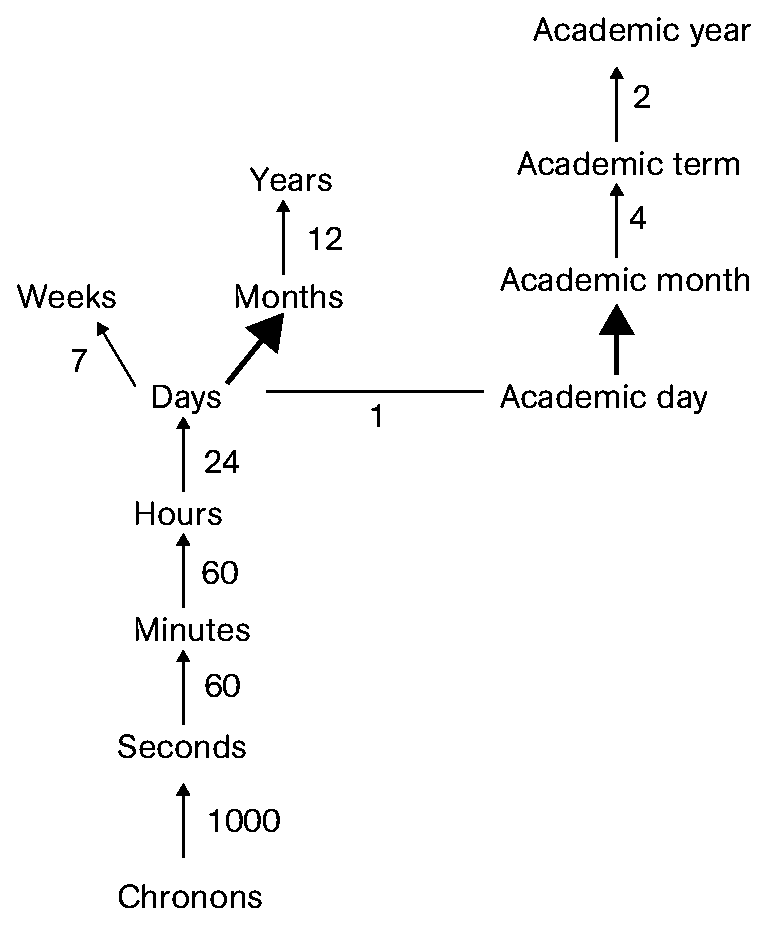
\includegraphics[scale=0.5]{graphs/granularityGraph.eps}
\caption{The granularity graph corresponding to example~\ref{examplegrangraph}.}
\label{fig:granularity-graph-example}
\end{figure}

\vspace{-25pt}

%Next, in subsection \ref{subsec:timedomain-calendar}, some basic concepts and issues concerning calendars are explained.

%\subsection{Calendars}
%\label{subsec:timedomain-calendar}
%maybe introduce previously the concept of time units, linear hierarchy and time point.

%This subsection will concern \emph{calendars}. A calendar provides some sort of human interpretation of time. As such, calendars provide meaning or interpretation to temporal values where this meaning or interpretation is relevant or useful to the user. More precisely, calendars determine the mapping between human-meaningful time values and an underlying time model~\cite{Dyreson1994}. More formally, a calendar is an organization of different granularities (e.g., granularities day, month and year) in a hierarchy. In order to formally define what a calendar is, some other concepts should first be introduced~\cite{Kraus1997}:


%\begin{svgraybox}
%\vspace{-10pt}
%\begin{definition}\textbf{(Calendar)}\\
%A \emph{\textbf{calendar}} 
%\end{definition}
%\vspace{-10pt}
%\end{svgraybox}


%\begin{svgraybox}
%\vspace{-10pt}
%\begin{definition}\textbf{Linear Hierarchy of Granularities}\\
%A \emph{\textbf{linear hierarchy of granularities}} is a finite set of granularities with a linear order (denoted $\sqsubset$). The most coarse granularity is called \emph{the top of the hierarchy} and must be an infinite set while all other granularities must be finite sets.
%\end{definition}
%\vspace{-10pt}
%\end{svgraybox}

%An example of a linear hierarchy is the set $\left\{ \text{days, months, years} \right\}$, where days $\sqsubset$ months and months $\sqsubset$ years. With this, a \emph{linear calendar} can be defined.

%\begin{svgraybox}
%\vspace{-10pt}
%\begin{definition}\textbf{Linear Calendar}\\
%A \emph{\textbf{linear calendar}} consist of a linear hierarchy of granularities and a validity predicate which specifies if a granule is valid in the calendar.
%\end{definition}
%\vspace{-10pt}
%\end{svgraybox}

%An example of a linear calendar could be the linear hierarchy $\left\{ \text{days, months, years} \right\}$, where days $\sqsubset$ months and months $\sqsubset$ years, together with a validity predicate that excludes time indications like `32 April 2012' or `30 February 2012'.

%The linear hierarchy days $\sqsubset$ months $\sqsubset$ years represents a linear calendar. It is necessary to define the validity predicates because 17 January 2012 is a valid element of the calendar whereas 30 February 2012 is not.
 
%\textcolor{red}{CHECK}
%\subsubsection{\label{subsubsubsec:julian-day-number}An example of temporal domain: Julian Day Number}
%% proposal for the underlying Julian Day Number domain.
%
%The Julian Day number \emph{JDN} \cite{Dir96} is a counter. Its value is incremented in one unit every day from 1 January 4713 B.C. at 12:00 noon. The particularity of starting at noon was useful for astronomers: the observations they took one night belonged to the same Julian Day.\\
%Note that the Julian Day represents whole days. There is an extension that allows to represent any precision needed (it is called Julian Date). By default, a Julian Day is expressed in Universal Time. (U.T, also known as Solar Time). However, there are representations in Terrestrial Time (T.T), Epheris Time (J.E.D. or J.D.E.). Any time scale different from Universal Time must be explicit after the Julian Day number. There are several conversion formulas~\cite{Usn}\cite{Wik}\cite{Lea} between a date in Gregorian calendar  format and a date in  JDN format. The inverse conversion formula is proposed in~\cite{Fliegel:1968:LEM:364096.364097}\\
%
%There are many alternatives to optimize the representation of Julian Day numbers because of its extremely far origin (4713 B.C. year). Table \ref{table:juliandayrepresentations} shows several time domains that can be calculated from the Julian Date, some of them are proposed just for optimization purposes.
%
%
%\begin{table}
%\caption{Julian Day representations}
%\label{table:juliandayrepresentations}
%
%\begin{tabular}{p{2cm}p{4cm}p{4cm}p{2cm}}
%%header ------------------------------------------------------
%\hline\noalign{\smallskip}
%Name & From & Formula & Current Value  \\ 
%\noalign{\smallskip}\svhline\noalign{\smallskip}
%%header ------------------------------------------------------
%Julian Date (JD)$^a$ & 12:00 noon Monday 1 January 4713 B.C & & 2455278. 85488  \\ 
%Julian Day Number (JDN)$^b$ & 12:00 noon  Monday 1 January 4713 B.C. & JND = floor(JD) & 2455278 \\ 
%Reduced Julian Day (RJD)$^c$ & 12:00 noon Tuesday 16 November 1858 A.C. & RJD = JD - 2400000 & 55278.85488  \\ 
%Modified Julian Day (MJD)$^d$ & 00:00 Wednesday 17 November 1858 A.C. & MJD = JD - 2400000,5 & 55278.35488 \\ 
%Truncated Julian Day (TJD)$^e$ & 00:00 Friday 24 May 1968 A.C. & TJD = JD - 2440000,5 & 15278.35488  \\ 
%Truncated Julian Day (TJD)$^f$ & 00:00 Thursday 10 November 1995 A.C. & TJD = (JD- 0,5) mod 10000 & 5278. 35488   \\ 
%Dublin Julian Day (DJD))$^g$ & 12:00 noon Sunday 31 December 1899 A.C. & DJD = JD - 2415020 & 40258. 85488 \\ 
%Chronological Julian Day (CJD)$^h$  & 00:00 Monday 1 January 4713 B.C. & CJD = JD + 0,5 + timezone adjust. & 2455279. 3548843 (UT)  \\ 
%Lilian Day Number$^i$ & Friday 15 October 1582 & floor(JD-2299160,5) & 156118 \\ 
%ANSI Date$^j$  & Monday 1 January 1601 & floor(JD-2305812,5) & 149466  \\ 
%Rata die$^k$  & Monday 1 January 1 A.C & floor(JD - 1721424.5) & 733854 \\ 
%Unix time$^l$  & Thursday 1 January 1970 A.C. & (JD – 2440587.5) × 86400 & 1269333062 \\ 
%\noalign{\smallskip}\hline\noalign{\smallskip}
%\end{tabular}
%$^a$ This is an extension of the Julian Day that allows time representation. \\
%$^b$  Each day changes at noon. \\
%$^c$  Used by astronomers. \\
%$^d$ It starts at midnight. \\
%$^e$ Definition from NASA. \cite{Sch}. \\
%$^f$ Definition from NIST. \cite{Nis}. \\
%$g$ Introduced by the IAU in 1995. \\
%$^h$ The timezone must be explicited. Each day changes at midnight. \\
%$^i$ The number of days since Gregorian calendar in Universal Time. \\
%$^j$ The origin for COBOL integer dates. \\
%$^k$  The number of days since actual era. \\
%$^l$  It counts the seconds not the day. \\
%\end{table}
%
%\textcolor{red}{END CHECK}

%The next section briefly introduces temporal relationships.

\subsection{\label{allen-crisp}Temporal Relationships}
%an explanation on allen's temporal relations.
%definition of fuzzy temporal interval
In this section, a brief introduction can be found, concerning \emph{temporal relationships}, sometimes also called `temporal relations'\cite{Billiet:Pons:Matthe:DeTre:Pons:2011:BipolarFuzzy}. Temporal relationships can be seen as relationships between temporal elements belonging to the same time domain. These relationships express how the temporal elements are related to one another, with respect to temporal precedence and overlap.

\def\JPicScale{0.5}
\begin{figure}[h]
\centering
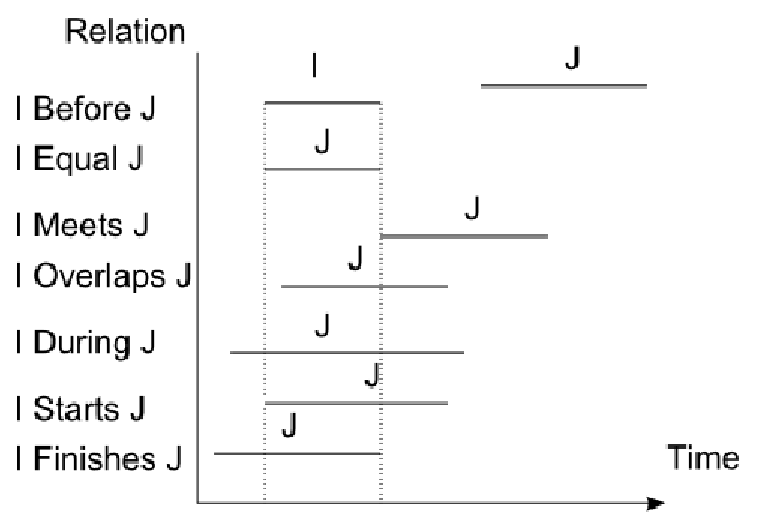
\includegraphics[scale=0.5]{graphs/allen.eps}
\caption{Allen relations between two time intervals I and J.}
\label{fig:allen}
\end{figure}

Several (collections of) operators have been proposed in order to compare temporal elements and model the temporal relationships between them. Allen~\cite{Allen83} most notably described such relationships between time intervals and as a special case, between instants. Figure~\ref{fig:allen} shows the temporal relationships Allen discerned. Some proposals can be applied to both crisp and other time intervals~\cite{ohlbach2004},~\cite{nagypal2003},~\cite{schockaert08},~\cite{garrido2009}.

%In the next section, some basic concepts and terminology about temporal databases are presented, followed by an overview of some interesting issues concerning temporal databases and a survey of some commercial temporal database systems.

\section{Temporal Databases}
\label{sec:temporal-databases}
%
% Temporal databases
%
This section defines the model used to represent time in a database. This model allows working with time instants and time intervals.  Even though there is no general agreement as to whether real-time line is continuous or discrete, a discrete model of time may be the most appropriate for a temporal database. 

	A chronon may be defined as the basic unit of time. Mathematically, a chronon is isomorphic to a finite sequence of natural numbers. For instance, if a chronon is \emph{11232010}, it represents a day, namely 11/23/2010. The symbol \emph{c} denotes a chronon. A chronon may represent different time granularity, depending on database or user processing needs (i.e. minutes, seconds, milliseconds, etc.). Real-time instants are smaller than chronons even though they are represented by the said chronons The real-time line is represented by a finite sequence of chronons. 

	It is possible to represent time intervals by a sequence of consecutive chronons. A sequence of consecutive chronons could be represented by the pair of starting and terminating chronons. A restriction must be imposed so that the starting instant comes before the ending instant.
\subsubsection{Temporal data models and time domains}
\label{sec:temporaldatamodelsandtimedomains}
A temporal data model is a relational data model which has temporal relations as underlying data structure, and whose operators are all temporal. In \cite{Böhlen_point-versus}, a study between interval-based and point-based temporal data models is shown. We are going to explain the main definitions and the equivalence between the models.

Temporal relations include a temporal attribute. A tuple of a temporal relation may be put under the form $(x_1,...,x_n||t_s)$ where $(x_1,...,x_n)$ are the non-temporal attribute values and \emph{t} is the tuple timestamp. Furthermore, an operator is temporal only if it generates a temporal relation when it is applied to temporal relations.

	The choice of the timestamp representation of the database facts is an important factor. Two options are the most common choices: time points and time intervals. Time intervals may be built from time points. The definition of time point is the following:
Let T be an infinite set.

$T^p=\langle T,< \rangle$ is a time point domain over $T$ iff $<$ defines a total order on $T$. Each element of $T$ corresponds to a time point of $T^p$.

The definition of time interval is:

A time interval $I$ of $T^p$ is any connected subset of $T^p$.

$T^i = \langle I,\subset \rangle $ is the time interval domain over $T^p$ iff $I$ is the set of all the intervals of $T^p$.

Both $T^p$ and $T^i$ are time domains over $T$.

A timestamp over $T^p$ is either a time point or a time interval of $T^p$. Time intervals can be represented as sets of time points which may, in turn, be represented by a time interval with the same values at both of its ends. Sometimes a coalesce operator is defined so as to switch between a set of time points and a time interval. Logically, defining a un-coalescing operator is quite complex. 
\subsubsection{\label{subsubsec:timeDb}Time in databases}
We can classify the time recorded in the database through its semantics. As a result, two kinds of time derive from two orthogonal time domains: valid time and transaction time. Valid-time captures the time-varying nature of the reality model. Transaction time structures the update activity associated with the object. The resulting temporal relations are those emerging from the bitemporal conceptual data model BCDM, on which TSQL2 is based.

The domain of valid time is given as $D_{VT}=\lbrace{c_1^v,c_2^v,...,c_k^v}\rbrace$, whereas the domain of transaction time may be given by $D_{TT}=\lbrace{c_1^t,c_2^t,...,c_k^t}\rbrace$. Thus, a valid-time chronon $c^v$  is a member of $D_{VT}$, a transaction-time chronon $c^t$ is a member of $D_{TT}$ and a bitemporal chronon $c^b=(c^t,c^v)$ is an ordered pair of a transaction-time chronon and valid-time chronon.

We can define the set of names $D_A=\lbrace{A_1,A_2,...,A_n}\rbrace$as attributes and the following set of domains for the said attributes:$D_D=\lbrace{D_1,D_2,...,D_n}\rbrace$. We may also define $\bot_i$ as inapplicable,$\bot_u$ as unknown, and $\bot$ as inapplicable or unknown null values. 

The schema for a bitemporal relation $'R'$ consists of an arbitrary number of explicit attributes from $D_A$ with domains in $D_D$ and an implicit timestamp attribute $T$ with domain $2^{\lbrace D_{TT}\bigcup \lbrace UC \rbrace \cdot D_{VT}\rbrace}$, where $UC$ ('until changed') means that the tuple is current in the database. This schema is a special transaction-time marker.

A 'fact' is the information stored in a tuple. We define a tuple as $x=(a_1,a_2,...,a_n|t^b)$ in a bitemporal conceptual relation instance $r(R)$, which consists of a number of attribute values associated with a bitemporal timestamp value. A value $(UC,c^v)$ in a timestamp indicates that the tuple is current in the database.

We say that a fact is true in the reality model during each valid-time chronon when a subset of the valid-time domain is associated with that fact.

We say that a fact is current in the relation during each transaction-time chronon when a subset of the transaction-time chronon domain is associated with the valid-time chronon. Only the subset of transaction times less than UC may be associated with a valid time.

While the definition of a bitemporal chronon is symmetric, the relation between valid time and transaction time is asymmetric. It should also be noted that since no two tuples with identical attribute values are allowed in a bitemporal relation instance, the full history of a fact is contained in a single tuple. In graphical representations of bitemporal space, the x-axis represents the transaction-time dimension and the y-axis denotes the valid-time dimension.

There are two special cases of bitemporal relations:
\begin{itemize}
\item
Valid-time relations, which support only valid time.
\item
Transaction-time relations,which support only transaction time.
\end{itemize}
We use the term 'snapshot relation' for a conventional relation. This relation supports neither transaction nor valid time.
\subsubsection{Implicit versus explicit timestamps}
\label{sec:implicitversusexplicittimestamps}
The association between time and facts may be carried out in two ways: explicitly, where the relation is represented by fully explicit timestamps, and implicitly. This distinction is relevant to three aspects of the data model: the update language, the display of data and the query language.

	If the time model works with transaction time, it means that the update language contains implicit timestamps. The transaction-time chronons of the facts are supplied by the system; in the valid-time model, these chronons are supplied by the user. Thus, in a bitemporal data model, the chronons are also supplied by the user.

	If the time model allows displaying temporal facts, it must represent such data explicitly. It is possible that the model allows the user to choose between several representations of time. In some simple transaction-time models it is common that the temporal facts cannot be displayed. 

	The main difficulty about differentiating between implicit and explicit timestamps is the query language. By means of the query language, we may directly access temporal attributes: the temporal attributes are as explicit as the other attributes in the database. If the query language does not allow direct access to temporal attributes, the association schema between timestamps and facts is considered implicit.
	
\subsubsection{\label{subsubsec:models}Temporal data models}
There are several extensions to the relational model that include the temporal element. In the current section, we briefly describe the model and some of its most interesting features. A more detailed summary can be found in \ref{sec:timeindatabasedesign}. Some models work only with valid or transaction time, whereas a few models can handle both. The current study starts with the models supporting valid time only, continues through the models which support transaction time and finally deals with the bitemporal models.

\paragraph{Valid-time models}
Most models support valid time only.

Brooks:  \cite{brooks56} Proposes a tridimensional view of valid-time database.

Wiederhold: \cite{Blum:1981:DCD:1672611.1672632} Time-oriented database, developed to work with medical applications. This model depicts relations as sets of entity-attribute-time-value quadruples. Time is associated with the visit number of the patient. 

Jones LEGOL 2.0: \cite{legol20} A language used in legislative writing. The temporal order of elements and the valid times for objects are important. It was the first time-oriented algebra to be defined, and some of its features are found in subsequent algebras.
Tuples in this model have two time attributes: Start and Stop. Each one indicates the start point and the end point of the interval where the tuple is valid.

Clifford-1: \cite{Clifford82},\cite{Clifford:1983:FST:319983.319986} Each relation schema has an additional time value called 'State'. Also, a boolean attribute is added to indicate if this tuple exists for that state.

Ariav: \cite{Ariav:1986:TOD:7239.7350} Temporally-oriented data model: a valid-time relation is a set of snapshot relation states indexed by valid time. A calculus-based query language is associated with the model: TOSQL.

Navathe: \cite{TSQL} Proposes a temporal extension to SQL called TSQL, the temporal algebra associated to the temporal relational model. This model allows a relationship to handle time-varying attributes, and also relationships without time-varying attributes. The only restriction is that all attributes in the relation must be of the same type. Objects are classified in snapshot relations and valid-time relations. In the latter, each tuple has associated to it an interval of validity with two points: time-start and time-end, like in the LEGOL 2.0 model.

Sadeghi: \cite{913787} Proposes a calculus-based valid-time language, HQL, where all objects represent valid-.time relations. As in Navathe and LEGOL 2.0, two time points are required for the ends of the interval. The model requires coalescing.

Sarda: \cite{Sarda:1990:ESH:627277.627409} This model was designed to support the calculus-based model HSQL. The model associates valid-time with tuples. Objects can either be snapshot or valid-time relations. In this model, valid time is considered to be closed on the left part of the interval and open on the right. Time is represented by an implicit attribute called 'Period' as a single non-atomic value.

The following time data models are not in first normal form (1NF), which means they might have multiple values per attribute. Even though these models are an extension of the 1NF, the representation is not in 1NF, but the operators work on valid-time relations, which are extensions of conventional relations.

Segev: \cite{Segev:1987:LMT:38714.38760} Defines the temporal data model, whose principal time structure is the time sequence. A time sequence is a surrogate value that identifies the object along with a sequence of time-value pairs. There are several types of time sequences depending on the semantics of the data represented. 

Clifford-2: \cite{Clifford:1987:HRD:645472.653241},\cite{Clifford:1985:AHR:971699.318922} This model is a refinement of the previous one presented by the same author. The data model allows two types of objects: a set of chronons, termed a lifespan, and a valid-time relation in which each attribute and tuple is assigned a lifespan. A tuple is an ordered value containing the tuple value and its lifespan. Attributes are not atomic since an attribute value in a tuple is a partial function from the chronons' domain to the value domain of the attribute. Relations have key attributes and, at the same chronon, no two tuples are allowed to match the key attributes.


Tansel: \cite{Tansel:1986:ATD:23125.23132},\cite{Clifford:1985:AHR:971699.318922} Designed to support the calculus-based query language (Hquel) and the time by example language. The model supports only one type of object: the valid-time relation. Four types of attributes are supported. If we take the time into account, attributes can be time-varying or non-time-varying. Then, attributes can be atomic-valued or set-valued. There is no need for attributes in the relation to be of the same type, and attribute values in a given tuple do not need to be homogeneous. A triplet containing an element from the attribute's value domain and the boundary points of the time interval represents the value of a time-varying atomic-valued attribute. A set-valued attribute is represented by a set of these triplets.

Gadia-1:  \cite{Gadia:1988:HRM:49346.50065},\cite{Gadia:1985:QLH:325405.325412} This homogeneous model allows two types of objects: valid-time elements and valid-time relations. The model requires that all attribute values in a given tuple be functions on the same valid-time element. Unlike intervals, valid-time elements are closed under union, difference, and complementation.
Bhargava presents an extension of this model to both valid and transaction time. 

Gadia-2: \cite{Gadia:1986:TMM:645471.655410},\cite{Chuen},\cite{Gadia:1988:GMR:971701.50233} Is an extension of the homogeneous model known as multihomogeneous model. Temporal elements may be multi-dimensional to model both valid and transaction time. Attribute values are functions from temporal elements onto attribute value domains, but attribute values do not need to be on the same temporal element. The key attributes in the relations must be single-valued in respect to the interval of validity. 

Lorentzos: \cite{springerlink:10.1007/3-540-19074-0_71},\cite{Lorentzos:1989:HDT:70777.70787} The temporal relational model allows to specify different granularities and the support of periodic events. This model associates timestamps with individual attribute values rather than with tuples. Timestamps are explicit values updated directly by the user. The said timestamps represent either the chronon during which attribute(s) were valid or a boundary point of the interval of validity. In the model, several timestamps of different granularities can be used together in the specification of a chronon.
This model has the particularity that some columns have a different meaning depending on the context.

\paragraph{Transaction-time models}
The main feature of the transaction-time models is that they are append-only.

Kimball: \cite{kim78} The temporal model is called DATA. In it, the association between facts and times is implicit. Also, the update operations avoid the explicit use of time. However, transaction-time relations cannot be displayed but can only be depicted in the snapshots extracted from the transaction-time relations. At query language level, the association of facts and times is also implicit.

Stonebraker: \cite{Ston87} Proposes the Postgres data model. Like in the previous model, the association between time and facts in the three model features (update language, query language and visualization) is implicit. In this model, the visualization is not restricted to snapshot relation states.
In this model, two timestamps are used when specifying the time for a given tuple that is current in the relation.

Jensen: \cite{Jensen:1991:IIM:627283.627484} In the DM/T model, the association of facts and times is also implicit. DM/T contains a backlog for each user-defined transaction-time relation. This backlog contains the full history of the associated user-defined transaction-time relation. When an insert, delete or update operation is performed, the backlog for this relation is updated.

\paragraph{Bitemporal data models}
The bitemporal data models support both valid and transaction time. This section deals with the following seven models of a bitemporal data model.

Ben-Zvi: \cite{910377} Proposed the time relational model,, which defines two types of objects: snapshot relations and bitemporal relations. Each tuple in a bitemporal relation has five additional implicit attributes:
The two interval ends of the valid-time chronon, called 'Effective-time-start' and 'Effective-time-stop'.
The two interval ends of the transaction-time chronon. 'Registration-time-start' is the transaction-time chronon associated with the 'Effective-time-start', 'Registration-time-stop' is the transaction-time chronon associated with the 'Effective-time-stop'.
Deletion-time. It registers when a tuple which was mistakenly entered is logically deleted.

Ahn: \cite{Snodgrass:1985:TTD:318898.318921},\cite{sno86} This model follows a four-dimensional data model. Each instance is represented as a sequence where each value is composed by a timestamp with a transaction-time chronon and a three dimensional volumes -one of these dimensions being the valid time.

Snodgrass:  \cite{sno86},\cite{Snodgrass:1984:TQL:588011.588041} The data model has four implicit attributes: 
The transaction time when the tuple was inserted.
The transaction time when the tuple was deleted.
The starting point of the valid-time interval.
The end point of the valid time-interval.
	
	The data query language associated with the model is called TQuel.

McKenzie: \cite{Snodgrass:1993:ATQ:642875.642890},\cite{Mckenzie:1988:ALQ:915060}, \cite{mck81} In this model, the attribute's values are timestamped, but it is required that attributes be single-valued. This makes it possible to perform a Cartesian product. There are two types of objects in the model: the snapshot relations and the valid-time relations. Thus, transaction-time relations are modeled as sequences of snapshot relations. Bitemporal relations are sequences of valid-time relations indexed by transaction time. An attribute's value in a valid-time relation is an ordered pair: a value from the attribute's domain and a set of chronons. Relations are not allowed to have value-equivalent tuples. The model also allows the schema and even the class of the relation (snapshot, transaction-time, valid-time and bitemporal) to change.

Gadia-3: \cite{Bhargava:1993:RDS:642811.642819},\cite{gad92} This data model is associated with the calculus-based query language TempSQL. Attributes are timestamped with finite unions of rectangles in the valid-time x transaction-time space.

Thompson: \cite{171833} This model, based on an accounting system, is called Accounting Data Model. It has four timestamp attributes: two for transaction time, called 'engineering time', and two for valid time, called 'accounting time'. Also, a boolean value called 'timewarp' enables the attribute to change historically. 



\section{Imprecision, Uncertainty and vagueness in temporal databases}
\label{sec:imprecision-uncertainty}
%
% Fuzzy temporal databases
%
Some software applications deal with uncertainty related to time. e.g. a logistics company which transports packages from one destination to another. The time when the package would be at the end point may be stimated but not precisely known. These applications need to manage the uncertainty with respect to the temporal attributes of the objects stored in the database.

There are several approaches to manage uncertainty in the temporal information stored in a database. Valid-time is usually represented as an interval, and therefore it is suitable for the representation of uncertainty in the valid-time interval. Nevertheless, the values for transaction and decision time are usually precisely known.
Some models deal with probability~\cite{Dekhtyar2001} or possibility~\cite{Dubois89} distributions at the endpoints of the time interval. In this section we will explain the most interesting proposals that deal with possibility distributions in the valid-time interval. %Two are the main points developed within this section: the representation of uncertainty in the time interval and the flexible querying of ill-known time periods.

In fuzzy databases~\cite{Galindo2006}, uncertainty is managed at storage level whereas imprecision is managed at querying level. In subsection \ref{subsec:representation-time-intervals} we will explain the main approach for the storage of uncertainty in the valid-time interval. Finally, in subsection \ref{subsec:querying-time-intervals} the proposals for querying in a flexible way valid-time intervals are analyzed.

\subsection{Representation of ill-known temporal intervals}
\label{subsec:representation-time-intervals}
The uncertainty in a valid-time interval may be represented with uncertainty at one or both starting and ending points. The uncertainty is usually represented by means of a possibility distribution in one or both points. It is also possible to represent with rough sets~\cite{Pawlak1995} time intervals~\cite{Qia09}.

Several authors ~\cite{garrido2009} propose some transformations in order to optimize the storage of the valid-time interval. Further research has shown how these transformations drive to a possibilistic information lost~\cite{Pon11}. A comparison between the transformations in ~\cite{garrido2009}  and the framework in~\cite{Pon11} is done in~\cite{pon12}. 

\begin{figure}
\centering
%%Created by jPicEdt 1.4.1_03: mixed JPIC-XML/LaTeX format
%%Wed Nov 23 16:38:02 CET 2011
%%Begin JPIC-XML
%<?xml version="1.0" standalone="yes"?>
%<jpic x-min="-2.5" x-max="60" y-min="-2.5" y-max="32.5" auto-bounding="true">
%<multicurve fill-style= "none"
%	 points= "(0,0);(0,0);(55,0);(55,0)"
%	 right-arrow= "head"
%	 />
%<multicurve fill-style= "none"
%	 points= "(0,0);(0,0);(0,30);(0,30)"
%	 right-arrow= "head"
%	 />
%<text fill-style= "none"
%	 text-vert-align= "center-v"
%	 anchor-point= "(-2.5,27.5)"
%	 text-frame= "noframe"
%	 text-hor-align= "center-h"
%	 right-arrow= "head"
%	 >
%1
%</text>
%<text fill-style= "none"
%	 text-vert-align= "center-v"
%	 anchor-point= "(-2.5,0)"
%	 text-frame= "noframe"
%	 text-hor-align= "center-h"
%	 right-arrow= "head"
%	 >
%0
%</text>
%<text fill-style= "none"
%	 text-vert-align= "center-v"
%	 anchor-point= "(15,32.5)"
%	 text-rotation= "135"
%	 text-frame= "noframe"
%	 text-hor-align= "center-h"
%	 right-arrow= "head"
%	 >
%Membership Degree
%</text>
%<text fill-style= "none"
%	 text-vert-align= "center-v"
%	 anchor-point= "(10,-2.5)"
%	 text-frame= "noframe"
%	 text-hor-align= "center-h"
%	 right-arrow= "head"
%	 >
%2
%</text>
%<text fill-style= "none"
%	 text-vert-align= "center-v"
%	 anchor-point= "(15,-2.5)"
%	 text-frame= "noframe"
%	 text-hor-align= "center-h"
%	 right-arrow= "head"
%	 >
%3
%</text>
%<text fill-style= "none"
%	 text-vert-align= "center-v"
%	 anchor-point= "(20,-2.5)"
%	 text-frame= "noframe"
%	 text-hor-align= "center-h"
%	 right-arrow= "head"
%	 >
%4
%</text>
%<text fill-style= "none"
%	 text-vert-align= "center-v"
%	 anchor-point= "(25,-2.5)"
%	 text-frame= "noframe"
%	 text-hor-align= "center-h"
%	 right-arrow= "head"
%	 >
%5
%</text>
%<text fill-style= "none"
%	 text-vert-align= "center-v"
%	 anchor-point= "(30,-2.5)"
%	 text-frame= "noframe"
%	 text-hor-align= "center-h"
%	 right-arrow= "head"
%	 >
%6
%</text>
%<text fill-style= "none"
%	 text-vert-align= "center-v"
%	 anchor-point= "(35,-2.5)"
%	 text-frame= "noframe"
%	 text-hor-align= "center-h"
%	 right-arrow= "head"
%	 >
%7
%</text>
%<text fill-style= "none"
%	 text-vert-align= "center-v"
%	 anchor-point= "(40,-2.5)"
%	 text-frame= "noframe"
%	 text-hor-align= "center-h"
%	 right-arrow= "head"
%	 >
%8
%</text>
%<text fill-style= "none"
%	 text-vert-align= "center-v"
%	 anchor-point= "(45,-2.5)"
%	 text-frame= "noframe"
%	 text-hor-align= "center-h"
%	 right-arrow= "head"
%	 >
%9
%</text>
%<text fill-style= "none"
%	 text-vert-align= "center-v"
%	 anchor-point= "(50,-2.5)"
%	 text-frame= "noframe"
%	 text-hor-align= "center-h"
%	 right-arrow= "head"
%	 >
%10
%</text>
%<text fill-style= "none"
%	 text-vert-align= "center-v"
%	 anchor-point= "(5,-2.5)"
%	 text-frame= "noframe"
%	 text-hor-align= "center-h"
%	 right-arrow= "head"
%	 >
%1
%</text>
%<multicurve fill-style= "none"
%	 points= "(5,0);(5,0);(15,27.5);(15,27.5)"
%	 />
%<multicurve fill-style= "none"
%	 points= "(15,27.5);(15,27.5);(20,0);(20,0)"
%	 />
%<multicurve fill-style= "none"
%	 points= "(25,0);(25,0);(35,27.5);(35,27.5)"
%	 />
%<multicurve fill-style= "none"
%	 points= "(35,27.5);(35,27.5);(50,0);(50,0)"
%	 />
%<text fill-style= "none"
%	 text-vert-align= "center-v"
%	 anchor-point= "(10,25)"
%	 text-frame= "noframe"
%	 text-hor-align= "center-h"
%	 >
%X
%</text>
%<text fill-style= "none"
%	 text-vert-align= "center-v"
%	 anchor-point= "(40,25)"
%	 text-frame= "noframe"
%	 text-hor-align= "center-h"
%	 >
%Y
%</text>
%<text fill-style= "none"
%	 text-vert-align= "center-v"
%	 anchor-point= "(60,0)"
%	 text-frame= "noframe"
%	 text-hor-align= "center-h"
%	 >
%Time
%</text>
%</jpic>
%%End JPIC-XML
%LaTeX-picture environment using emulated lines and arcs
%You can rescale the whole picture (to 80% for instance) by using the command \def\JPicScale{0.8}
\ifx\JPicScale\undefined\def\JPicScale{1}\fi
\unitlength \JPicScale mm
\begin{picture}(60,32.5)(0,0)
\linethickness{0.3mm}
\put(0,0){\line(1,0){55}}
\put(55,0){\vector(1,0){0.12}}
\linethickness{0.3mm}
\put(0,0){\line(0,1){30}}
\put(0,30){\vector(0,1){0.12}}
\put(-2.5,27.5){\makebox(0,0)[cc]{1}}

\put(-2.5,0){\makebox(0,0)[cc]{0}}

\put(15,32.5){\makebox(0,0)[cc]{Membership Degree}}

\put(10,-2.5){\makebox(0,0)[cc]{2}}

\put(15,-2.5){\makebox(0,0)[cc]{3}}

\put(20,-2.5){\makebox(0,0)[cc]{4}}

\put(25,-2.5){\makebox(0,0)[cc]{5}}

\put(30,-2.5){\makebox(0,0)[cc]{6}}

\put(35,-2.5){\makebox(0,0)[cc]{7}}

\put(40,-2.5){\makebox(0,0)[cc]{8}}

\put(45,-2.5){\makebox(0,0)[cc]{9}}

\put(50,-2.5){\makebox(0,0)[cc]{10}}

\put(5,-2.5){\makebox(0,0)[cc]{1}}

\linethickness{0.3mm}
\multiput(5,0)(0.12,0.33){83}{\line(0,1){0.33}}
\linethickness{0.3mm}
\multiput(15,27.5)(0.12,-0.65){42}{\line(0,-1){0.65}}
\linethickness{0.3mm}
\multiput(25,0)(0.12,0.33){83}{\line(0,1){0.33}}
\linethickness{0.3mm}
\multiput(35,27.5)(0.12,-0.22){125}{\line(0,-1){0.22}}
\put(10,25){\makebox(0,0)[cc]{X}}

\put(40,25){\makebox(0,0)[cc]{Y}}

\put(60,0){\makebox(0,0)[cc]{Time}}

\end{picture}

\caption{Two ill-known values $X$ and $Y$, represented by means of triangular possibility distributions denoting the starting and ending points of an ill-known interval. }
\label{fig:interval}
\end{figure}


An ill-known temporal interval is usually represented by means of two possibility distributions one in each starting and ending points. Figure \ref{fig:interval} shows an ill-known valid-time interval. The starting and ending points are denoted by two fuzzy numbers, $X$ and $Y$, represented by means of two triangular possibility distributions (see the Appendix). For illustration, figure \ref{fig:convexhull} shows one of the transformations based in the convex hull and proposed in~\cite{garrido2009}.

\begin{figure}
\centering
%%Created by jPicEdt 1.4.1_03: mixed JPIC-XML/LaTeX format
%%Mon Nov 28 16:07:12 CET 2011
%%Begin JPIC-XML
%<?xml version="1.0" standalone="yes"?>
%<jpic x-min="-2.5" x-max="60" y-min="-2.5" y-max="72.5" auto-bounding="true">
%<multicurve fill-style= "none"
%	 points= "(0,40);(0,40);(55,40);(55,40)"
%	 right-arrow= "head"
%	 />
%<multicurve fill-style= "none"
%	 points= "(0,40);(0,40);(0,70);(0,70)"
%	 right-arrow= "head"
%	 />
%<text text-vert-align= "center-v"
%	 anchor-point= "(-2.5,67.5)"
%	 fill-style= "none"
%	 text-frame= "noframe"
%	 text-hor-align= "center-h"
%	 right-arrow= "head"
%	 >
%1
%</text>
%<text text-vert-align= "center-v"
%	 anchor-point= "(-2.5,40)"
%	 fill-style= "none"
%	 text-frame= "noframe"
%	 text-hor-align= "center-h"
%	 right-arrow= "head"
%	 >
%0
%</text>
%<text text-vert-align= "center-v"
%	 anchor-point= "(15,72.5)"
%	 fill-style= "none"
%	 text-rotation= "135"
%	 text-frame= "noframe"
%	 text-hor-align= "center-h"
%	 right-arrow= "head"
%	 >
%Membership Degree
%</text>
%<text text-vert-align= "center-v"
%	 anchor-point= "(10,37.5)"
%	 fill-style= "none"
%	 text-frame= "noframe"
%	 text-hor-align= "center-h"
%	 right-arrow= "head"
%	 >
%2
%</text>
%<text text-vert-align= "center-v"
%	 anchor-point= "(15,37.5)"
%	 fill-style= "none"
%	 text-frame= "noframe"
%	 text-hor-align= "center-h"
%	 right-arrow= "head"
%	 >
%3
%</text>
%<text text-vert-align= "center-v"
%	 anchor-point= "(20,37.5)"
%	 fill-style= "none"
%	 text-frame= "noframe"
%	 text-hor-align= "center-h"
%	 right-arrow= "head"
%	 >
%4
%</text>
%<text text-vert-align= "center-v"
%	 anchor-point= "(25,37.5)"
%	 fill-style= "none"
%	 text-frame= "noframe"
%	 text-hor-align= "center-h"
%	 right-arrow= "head"
%	 >
%5
%</text>
%<text text-vert-align= "center-v"
%	 anchor-point= "(30,37.5)"
%	 fill-style= "none"
%	 text-frame= "noframe"
%	 text-hor-align= "center-h"
%	 right-arrow= "head"
%	 >
%6
%</text>
%<text text-vert-align= "center-v"
%	 anchor-point= "(35,37.5)"
%	 fill-style= "none"
%	 text-frame= "noframe"
%	 text-hor-align= "center-h"
%	 right-arrow= "head"
%	 >
%7
%</text>
%<text text-vert-align= "center-v"
%	 anchor-point= "(40,37.5)"
%	 fill-style= "none"
%	 text-frame= "noframe"
%	 text-hor-align= "center-h"
%	 right-arrow= "head"
%	 >
%8
%</text>
%<text text-vert-align= "center-v"
%	 anchor-point= "(45,37.5)"
%	 fill-style= "none"
%	 text-frame= "noframe"
%	 text-hor-align= "center-h"
%	 right-arrow= "head"
%	 >
%9
%</text>
%<text text-vert-align= "center-v"
%	 anchor-point= "(50,37.5)"
%	 fill-style= "none"
%	 text-frame= "noframe"
%	 text-hor-align= "center-h"
%	 right-arrow= "head"
%	 >
%10
%</text>
%<text text-vert-align= "center-v"
%	 anchor-point= "(5,37.5)"
%	 fill-style= "none"
%	 text-frame= "noframe"
%	 text-hor-align= "center-h"
%	 right-arrow= "head"
%	 >
%1
%</text>
%<multicurve fill-style= "none"
%	 points= "(5,40);(5,40);(15,67.5);(15,67.5)"
%	 />
%<multicurve fill-style= "none"
%	 points= "(15,67.5);(15,67.5);(20,40);(20,40)"
%	 />
%<multicurve fill-style= "none"
%	 points= "(25,40);(25,40);(35,67.5);(35,67.5)"
%	 />
%<multicurve fill-style= "none"
%	 points= "(35,67.5);(35,67.5);(50,40);(50,40)"
%	 />
%<text text-vert-align= "center-v"
%	 anchor-point= "(10,65)"
%	 fill-style= "none"
%	 text-frame= "noframe"
%	 text-hor-align= "center-h"
%	 >
%X
%</text>
%<text text-vert-align= "center-v"
%	 anchor-point= "(40,65)"
%	 fill-style= "none"
%	 text-frame= "noframe"
%	 text-hor-align= "center-h"
%	 >
%Y
%</text>
%<text text-vert-align= "center-v"
%	 anchor-point= "(60,40)"
%	 fill-style= "none"
%	 text-frame= "noframe"
%	 text-hor-align= "center-h"
%	 >
%Time
%</text>
%<multicurve fill-style= "none"
%	 points= "(0,0);(0,0);(55,0);(55,0)"
%	 right-arrow= "head"
%	 />
%<multicurve fill-style= "none"
%	 points= "(0,0);(0,0);(0,30);(0,30)"
%	 right-arrow= "head"
%	 />
%<text text-vert-align= "center-v"
%	 anchor-point= "(-2.5,27.5)"
%	 fill-style= "none"
%	 text-frame= "noframe"
%	 text-hor-align= "center-h"
%	 right-arrow= "head"
%	 >
%1
%</text>
%<text text-vert-align= "center-v"
%	 anchor-point= "(-2.5,0)"
%	 fill-style= "none"
%	 text-frame= "noframe"
%	 text-hor-align= "center-h"
%	 right-arrow= "head"
%	 >
%0
%</text>
%<text text-vert-align= "center-v"
%	 anchor-point= "(15,32.5)"
%	 fill-style= "none"
%	 text-rotation= "135"
%	 text-frame= "noframe"
%	 text-hor-align= "center-h"
%	 right-arrow= "head"
%	 >
%Membership Degree
%</text>
%<text text-vert-align= "center-v"
%	 anchor-point= "(10,-2.5)"
%	 fill-style= "none"
%	 text-frame= "noframe"
%	 text-hor-align= "center-h"
%	 right-arrow= "head"
%	 >
%2
%</text>
%<text text-vert-align= "center-v"
%	 anchor-point= "(15,-2.5)"
%	 fill-style= "none"
%	 text-frame= "noframe"
%	 text-hor-align= "center-h"
%	 right-arrow= "head"
%	 >
%3
%</text>
%<text text-vert-align= "center-v"
%	 anchor-point= "(20,-2.5)"
%	 fill-style= "none"
%	 text-frame= "noframe"
%	 text-hor-align= "center-h"
%	 right-arrow= "head"
%	 >
%4
%</text>
%<text text-vert-align= "center-v"
%	 anchor-point= "(25,-2.5)"
%	 fill-style= "none"
%	 text-frame= "noframe"
%	 text-hor-align= "center-h"
%	 right-arrow= "head"
%	 >
%5
%</text>
%<text text-vert-align= "center-v"
%	 anchor-point= "(30,-2.5)"
%	 fill-style= "none"
%	 text-frame= "noframe"
%	 text-hor-align= "center-h"
%	 right-arrow= "head"
%	 >
%6
%</text>
%<text text-vert-align= "center-v"
%	 anchor-point= "(35,-2.5)"
%	 fill-style= "none"
%	 text-frame= "noframe"
%	 text-hor-align= "center-h"
%	 right-arrow= "head"
%	 >
%7
%</text>
%<text text-vert-align= "center-v"
%	 anchor-point= "(40,-2.5)"
%	 fill-style= "none"
%	 text-frame= "noframe"
%	 text-hor-align= "center-h"
%	 right-arrow= "head"
%	 >
%8
%</text>
%<text text-vert-align= "center-v"
%	 anchor-point= "(45,-2.5)"
%	 fill-style= "none"
%	 text-frame= "noframe"
%	 text-hor-align= "center-h"
%	 right-arrow= "head"
%	 >
%9
%</text>
%<text text-vert-align= "center-v"
%	 anchor-point= "(50,-2.5)"
%	 fill-style= "none"
%	 text-frame= "noframe"
%	 text-hor-align= "center-h"
%	 right-arrow= "head"
%	 >
%10
%</text>
%<text text-vert-align= "center-v"
%	 anchor-point= "(5,-2.5)"
%	 fill-style= "none"
%	 text-frame= "noframe"
%	 text-hor-align= "center-h"
%	 right-arrow= "head"
%	 >
%1
%</text>
%<multicurve fill-style= "none"
%	 points= "(5,0);(5,0);(15,27.5);(15,27.5)"
%	 />
%<multicurve fill-style= "none"
%	 points= "(15,27.5);(15,27.5);(35,27.5);(35,27.5)"
%	 />
%<multicurve fill-style= "none"
%	 points= "(35,27.5);(35,27.5);(50,0);(50,0)"
%	 />
%<text text-vert-align= "center-v"
%	 anchor-point= "(60,0)"
%	 fill-style= "none"
%	 text-frame= "noframe"
%	 text-hor-align= "center-h"
%	 >
%Time
%</text>
%<text text-vert-align= "center-v"
%	 stroke-dasharray= "1;1"
%	 anchor-point= "(40,25)"
%	 stroke-style= "dashed"
%	 fill-style= "none"
%	 text-frame= "noframe"
%	 text-hor-align= "center-h"
%	 >
%T
%</text>
%</jpic>
%%End JPIC-XML
%LaTeX-picture environment using emulated lines and arcs
%You can rescale the whole picture (to 80% for instance) by using the command \def\JPicScale{0.8}
\ifx\JPicScale\undefined\def\JPicScale{1}\fi
\unitlength \JPicScale mm
\begin{picture}(60,72.5)(0,0)
\linethickness{0.3mm}
\put(0,40){\line(1,0){55}}
\put(55,40){\vector(1,0){0.12}}
\linethickness{0.3mm}
\put(0,40){\line(0,1){30}}
\put(0,70){\vector(0,1){0.12}}
\put(-2.5,67.5){\makebox(0,0)[cc]{1}}

\put(-2.5,40){\makebox(0,0)[cc]{0}}

\put(15,72.5){\makebox(0,0)[cc]{Membership Degree}}

\put(10,37.5){\makebox(0,0)[cc]{2}}

\put(15,37.5){\makebox(0,0)[cc]{3}}

\put(20,37.5){\makebox(0,0)[cc]{4}}

\put(25,37.5){\makebox(0,0)[cc]{5}}

\put(30,37.5){\makebox(0,0)[cc]{6}}

\put(35,37.5){\makebox(0,0)[cc]{7}}

\put(40,37.5){\makebox(0,0)[cc]{8}}

\put(45,37.5){\makebox(0,0)[cc]{9}}

\put(50,37.5){\makebox(0,0)[cc]{10}}

\put(5,37.5){\makebox(0,0)[cc]{1}}

\linethickness{0.3mm}
\multiput(5,40)(0.12,0.33){83}{\line(0,1){0.33}}
\linethickness{0.3mm}
\multiput(15,67.5)(0.12,-0.65){42}{\line(0,-1){0.65}}
\linethickness{0.3mm}
\multiput(25,40)(0.12,0.33){83}{\line(0,1){0.33}}
\linethickness{0.3mm}
\multiput(35,67.5)(0.12,-0.22){125}{\line(0,-1){0.22}}
\put(10,65){\makebox(0,0)[cc]{X}}

\put(40,65){\makebox(0,0)[cc]{Y}}

\put(60,40){\makebox(0,0)[cc]{Time}}

\linethickness{0.3mm}
\put(0,0){\line(1,0){55}}
\put(55,0){\vector(1,0){0.12}}
\linethickness{0.3mm}
\put(0,0){\line(0,1){30}}
\put(0,30){\vector(0,1){0.12}}
\put(-2.5,27.5){\makebox(0,0)[cc]{1}}

\put(-2.5,0){\makebox(0,0)[cc]{0}}

\put(15,32.5){\makebox(0,0)[cc]{Membership Degree}}

\put(10,-2.5){\makebox(0,0)[cc]{2}}

\put(15,-2.5){\makebox(0,0)[cc]{3}}

\put(20,-2.5){\makebox(0,0)[cc]{4}}

\put(25,-2.5){\makebox(0,0)[cc]{5}}

\put(30,-2.5){\makebox(0,0)[cc]{6}}

\put(35,-2.5){\makebox(0,0)[cc]{7}}

\put(40,-2.5){\makebox(0,0)[cc]{8}}

\put(45,-2.5){\makebox(0,0)[cc]{9}}

\put(50,-2.5){\makebox(0,0)[cc]{10}}

\put(5,-2.5){\makebox(0,0)[cc]{1}}

\linethickness{0.3mm}
\multiput(5,0)(0.12,0.33){83}{\line(0,1){0.33}}
\linethickness{0.3mm}
\put(15,27.5){\line(1,0){20}}
\linethickness{0.3mm}
\multiput(35,27.5)(0.12,-0.22){125}{\line(0,-1){0.22}}
\put(60,0){\makebox(0,0)[cc]{Time}}

\put(40,25){\makebox(0,0)[cc]{T}}

\end{picture}

\caption{Transformation based in the convex hull from the two ill-known points $X$ and $Y$. }
\label{fig:convexhull}
\end{figure}

\subsection{Querying fuzzy temporal databases}
\label{subsec:querying-time-intervals}



\subsubsection{Bipolarity in temporal database querying}

\section{Bipolarity on temporal databases}
\label{sec:bipolarity}
\input{sources/bipolarity.tex}

\section{Further research work}
\label{sec:further-research-work}
In this work we have presented the main properties of the time in an information system. An overview of the commercial temporal DBMS has also been introduced. Although, to the best of our knowledge, no commercial fuzzy temporal DBMS have been found.  Finally the managing of imprecision in temporal databases is explained. A brief introduction of bipolar querying in temporal databases is done at the end of the section. 

Further research work should be done in several ways: first of all, a theoretical model for both dealing with uncertainty in the database as well as in the querying should be defined. Then, another interesting work is to propose an implementation with both DDL (Data Definition Language) and DML (Data Manipulation Language).

\section*{Acknowledgements}
Part of this research is supported by the grant BES-2009-013805 within the research project TIN2008-02066: \emph{Fuzzy Temporal Information treatment in relational DBMS}.



\input{referenc}
\end{document}
